%% Copernicus Publications Manuscript Preparation Template for LaTeX Submissions
%% ---------------------------------
%% This template should be used for copernicus.cls
%% The class file and some style files are bundled in the Copernicus Latex Package, which can be downloaded from the different journal webpages.
%% For further assistance please contact Copernicus Publications at: production@copernicus.org
%% http://publications.copernicus.org/for_authors/manuscript_preparation.html


%% Please use the following documentclass and journal abbreviations for discussion papers and final revised papers.


%% 2-Column Papers and Discussion Papers
\documentclass[gmd,manuscript]{copernicus}



%% Journal Abbreviations (Please use the same for Discussion Papers and Final Revised Papers)

% Archives Animal Breeding (aab)
% Atmospheric Chemistry and Physics (acp)
% Advances in Geosciences (adgeo)
% Advances in Statistical Climatology, Meteorology and Oceanography (ascmo)
% Annales Geophysicae (angeo)
% ASTRA Proceedings (ap)
% Atmospheric Measurement Techniques (amt)
% Advances in Radio Science (ars)
% Advances in Science and Research (asr)
% Biogeosciences (bg)
% Climate of the Past (cp)
% Drinking Water Engineering and Science (dwes)
% Earth System Dynamics (esd)
% Earth Surface Dynamics (esurf)
% Earth System Science Data (essd)
% Fossil Record (fr)
% Geographica Helvetica (gh)
% Geoscientific Instrumentation, Methods and Data Systems (gi)
% Geoscientific Model Development (gmd)
% Geothermal Energy Science (gtes)
% Hydrology and Earth System Sciences (hess)
% History of Geo- and Space Sciences (hgss)
% Journal of Sensors and Sensor Systems (jsss)
% Mechanical Sciences (ms)
% Natural Hazards and Earth System Sciences (nhess)
% Nonlinear Processes in Geophysics (npg)
% Ocean Science (os)
% Proceedings of the International Association of Hydrological Sciences (piahs)
% Primate Biology (pb)
% Scientific Drilling (sd)
% SOIL (soil)
% Solid Earth (se)
% The Cryosphere (tc)
% Web Ecology (we)
% Wind Energy Science (wes)


%% \usepackage commands included in the copernicus.cls:
%\usepackage[german, english]{babel}
\usepackage{tabularx}
\usepackage{cancel}
\usepackage{multirow}
\usepackage{supertabular}
\usepackage{algorithmic}
\usepackage{algorithm}
\usepackage{amsthm}
\usepackage{float}
\usepackage{subfig}
\usepackage{rotating}


% OWN MODIFICATIONS
% tabularx: vertical alignment (p - top, m - center, b - bottom) in multi-column tabularx cells
\def\tabularxcolumn#1{p{#1}} 
\newcolumntype{L}[1]{>{\hsize=#1\hsize\raggedright\arraybackslash}X}%
\newcolumntype{R}[1]{>{\hsize=#1\hsize\raggedleft\arraybackslash}X}%
\newcolumntype{C}[1]{>{\hsize=#1\hsize\centering\arraybackslash}X}%


% TODO: remove next lines before submission!
% package todonotes to highlight thing to be done during manuscript development
%  add note (default): \todo{your_note}
%  create todo list: \listoftodos
\setlength{\textwidth}{160mm} % shrink textwidth to make comments fit to page margin
\usepackage{xargs} % Use more than one optional parameter in a new command
\usepackage{xcolor}  % Coloured text etc. must be before package listings, if used
\definecolor{Goldenrod}{rgb}{.93,.68,.05}
\definecolor{OliveGreen}{cmyk}{.64,0,.95,.40}
\usepackage[colorinlistoftodos, textsize=scriptsize, prependcaption, shadow]{todonotes} % todo-Listen
% definitions for personal todonote style
\newcommandx{\TP}[2][1=]{\todo[linecolor=Goldenrod,backgroundcolor=Goldenrod!25,bordercolor=Goldenrod,#1]{Tobias:\\#2}}
\newcommandx{\AB}[2][1=]{\todo[linecolor=OliveGreen,backgroundcolor=OliveGreen!25,bordercolor=OliveGreen,#1]{Axel:\\#2}}
\newcommandx{\TF}[2][1=]{\todo[linecolor=blue,backgroundcolor=blue!25,bordercolor=blue,#1]{Till:\\#2}}

%\newcommandx{\unsure}[2][1=]{\todo[linecolor=red,backgroundcolor=red!25,bordercolor=red,#1]{#2}}
%\newcommandx{\change}[2][1=]{\todo[linecolor=blue,backgroundcolor=blue!25,bordercolor=blue,#1]{#2}}
%\newcommandx{\info}[2][1=]{\todo[linecolor=OliveGreen,backgroundcolor=OliveGreen!25,bordercolor=OliveGreen,#1]{#2}}





\begin{document}

%\title{-- MANUSCRIPT rev. \today{} -- \newline LUMP: Analysing the impacts of landscape discretisation on simulated streamflow dynamics using a newly developed R package}
%\title{-- MANUSCRIPT rev. \today{} -- \newline LUMP: Facilitating the implementation of landscape connectivity into hydrological models for large scale operation}
\title{-- MANUSCRIPT rev. \today{} -- \newline lumpR: An R package facilitating hillslope-based landscape discretisation for large-scale hydrological models}


% \Author[affil]{given_name}{surname}

\Author[]{Tobias}{Pilz}
\Author[]{Till}{Francke}
\Author[]{Axel}{Bronstert}

\affil[]{Institute of Earth and Environmental Science, University of Potsdam, Germany}

%% The [] brackets identify the author with the corresponding affiliation. 1, 2, 3, etc. should be inserted.



\runningtitle{LUMP: R package for model landscape discretisation}

\runningauthor{Pilz et al.}

\correspondence{Tobias Pilz (tpilz@uni-potsdam.de)}



\received{}
\pubdiscuss{} %% only important for two-stage journals
\revised{}
\accepted{}
\published{}

%% These dates will be inserted by Copernicus Publications during the typesetting process.


\firstpage{1}

\maketitle


\listoftodos

\vspace*{2cm}

\begin{abstract}
TEXT
\end{abstract}



\introduction  %% \introduction[modified heading if necessary]

Hydrological simulation models are important tools for gaining process understanding, forecasting of streamflow, supporting water managers, and climate and/or land-use change impact studies.
However, the lack of a unified theory in catchment hydrology led to a large number of competing models \citep[e.g.,][]{Weiler2015}.
These differ in terms of aim and scope, process representation and parametrisation, temporal resolution, and spatial discretisation.
The latter includes the size and shape of units where the model's underlying mathematical equations are solved.

The most straightforward procedure is the discretisation of the landscape into quadratic grid cells of equal size, commonly referred to as \emph{fully distributed} approach.
This, however, suffers from several drawbacks such as a high computational burden and large memory demands as well as limitations in representing landscape variability and processes at smaller scales than given by the grid's resolution.
Another strategy is to treat a hydrological catchment as a single unit, known as \emph{lumped} approach.
While being easy to implement along with simple and fast computable conceptual process representations this approach fails to adequately represent complex landscapes and process interactions leading to a deteriorated simulation of hydrological catchment behaviour.
Therefore, \emph{semi-distributed} approaches are usually the preferred choice in practical applications \citep[e.g.,][]{Kumar2010, Euser2015}.
Although no clear definition exists and sometimes termed as "distributed" approach, this family of discretisation typically consists of a hierarchical multi-level scheme dividing a hydrological basin into several subbasins which in turn contain irregularly shaped computational elements being hydrologically uniform entities \citep[e.g.,][]{Krysanova1998}.
It is therefore distributed in a way that hydrological processes are simulated at different locations in the study area taking into account distributed model input (such as meteorological forcing and landscape parameters) and producing spatially variable output (such as lateral and vertical water flows) but lumped as naturally heterogeneous though hydrologically similar areas are aggregated and parameterised in the same manner.\TP{Sufficient definition of term "semi-distributed"?}

In the last decades a large number of discretisation schemes for semi-distributed models has been developed tailored to various model structures and adapted to specific objectives and needs of modellers.
Along with that an even larger number of software solutions exists and it is a difficult task to decide for a specific model and discretisation approach and a programme for landscape pre-processing.
Therefore, the first objective of this paper is to provide an overview of landscape discretisation algorithms and software implementations for semi-distributed hydrological model application.

As will be further discussed in section \ref{sec:review}, hillslope-based modelling is an efficient semi-distributed strategy for the investigation of semi-arid landscapes and allows to represent heterogeneous runoff generation processes preserving hydrological connectivity.
However, so far only few computer programmes exist aiding in the pre-processing of hillslope-based models.
The second objective therefore is to present a new software package for the discretisation of the landscape into representative hillslopes.
The package aims to be model independent, user-friendly, free and open-source, applicable to large scales, and where the underlying algorithm should preserve hydrological connectivity and landscape characteristics along the hillslopes.
To facilitate implementation and be able directly connect to a \emph{Geographical Information System} (GIS) it was decided to build upon the free and in scientific contexts widely used scripting language R \citep{Rcoretream2015}.
The package is introduced and described in section \ref{sec:lump}.

The third objective of this study is to investigate the role of subjective user decisions during landscape discretisation on simulated streamflow.
To achieve this, an example application of the developed R package in combination with the \emph{Water Availability in Semi-Arid landscapes} (WASA) model \citep{Guentner2004b} in a semi-arid landscape in northeastern Brazil is presented.
A sensitivity analysis is employed to analyse the impact of user decisions and accompanying discretisation complexity on the model results (section \ref{sec:methods}).
Eventually, the findings of this study are discussed and conclusions are inferred (sections \ref{sec:discussion} and \ref{sec:conclusions}, respectively).




\section{Review of landscape discretisation schemes and software implementations}
\label{sec:review}

\subsection{Discretisation approaches in semi-distributed hydrological modelling}
\label{sec:review_approaches}
Landscapes are typically mapped using Digital Elevation Models (DEMs).
\emph{Contour-based} DEMs store terrain information as contour lines (or x, y coordinate pairs) of specific elevation \citep{Moore1988}.
\citet{Moore1991b} and \citet{Maurer1997} show example applications of contour-based terrain analysis for hydrological model application where this type of DEM proved to be powerful as its structure is based on the way how water flows on (albeit not necessarily below) the land surface.
However, although they have been further investigated for hydrological application \citep[e.g.,][]{Maunder1999, Moretti2008} contour-based DEMs come along with some limitations.
They have a relatively high data storage demand, topographic attributes are complicated to derive, and they provide no computational advantages \citep{Moore1991a}.
\emph{Triangulated Irregular Networks} (TINs) form a type of DEM sampling elevation points at specific landscape features, such as peaks or ridges, and form an irregular network of x, y, and z coordinates.
They are very flexible as, due to their irregular structure, they are able to map regions of high heterogeneity with more data points than smooth terrain and thus avoid redundancy and increase data storage efficiency \citep{Moore1991a, DeVantier1993}.
TINs also proved to be useful in a number of hydrological applications \citep[e.g.,][]{Tucker2001, Vivoni2004, Ivanov2004, Freitas2016}.
Their irregularity, however, makes the computation of topographic attributes more difficult and there can be problems when determining upslope connections for watershed derivation \citep{Moore1991a}.
\emph{Grid-based} DEMs store elevation information as a regularly spaced mesh.
There are a number of drawbacks as the regular structure might impose artefacts and discontinuities while sub-resolution landscape features cannot be captured limiting the applicability for hydrological purposes.
Furthermore, when increasing the grid's resolution to reduce these problems, computational burden and memory requirements are increased reducing their suitability for large scale applications.
Nevertheless, grid-based DEMs are the most widely used data structures due to their straightforward generation from remote sensing data, direct applicability for further investigations, and efficient calculation of geomorphological characteristics \citep{Moore1991a, DeVantier1993}.

As as basis for watershed delineation and further landscape discretisation, a number of pre-processing steps have to be performed.
This typically includes \emph{(i)} pit-filling of the DEM to remove sink areas and ensure a proper drainage of water from the catchment;
\emph{(ii)} computation of flow directions;
\emph{(iii)} computing upslope contributing area (i.e., the accumulated flow for each DEM unit);
\emph{(iv)} derivation of the river network, typically based on flow accumulation from the previous step;
\emph{(v)} delineation of the hydrological basin and subbasins.
For each step different algorithms have been proposed whose selection depends on the type of DEM, model to be employed, aim and scope of the study, or just personal preferences, e.g., in terms of software to be used \citep[e.g.,][]{OCallaghan1984, Tarboton1991, Costa-Cabral1994, Lacroix2002, Vivoni2004, Moretti2008}.

There exists a large number of landscape discretisation schemes for semi-distributed \TP{Definition of term "semi-distributed" in Introduction sufficient?} hydrological model application.
Some models explicitly use TINs, such as tRIBS \citep{Ivanov2004}, or modelling units derived from contour-based DEMs, e.g., THALES \citep{Grayson1992}.
The majority, however, delineate irregularly shaped polygons as computational model units derived from grid-based DEMs.

\citet{Wood1988} defined the smallest discernible averaging watershed where statistics of runoff generation did not further change as \emph{Representative Elementary Area} (REA) and applied simple conceptual equations for simulation of runoff generation.
They found the size of their REA to be primarily influenced by topography.
The concept of \emph{Hydrological Response Units} (HRUs), introduced by \citet{Leavesley1983} for their Precipitation-Runoff Modeling System (PRMS) and further elaborated by \citet{Fluegel1995}, is maybe the most prominent landscape discretisation scheme.
An HRU is assumed to be a homogeneous set of hydrological process dynamics formed by a pedo-topo-geological association with specific land-use and as such controlled by land-use management and physical landscape properties.
The conception has been adopted for a number of models such as SWAT \citep{Manguerra1998}, SWIM (therein termed \emph{hydrotopes}) \citep{Krysanova1998}, PREVAH \citep{Viviroli2009}, or GSFLOW \citep{Markstrom2008}.
MHYDAS is a process-based hydrological model for which the HRU concept has been further pursued for application in agricultural management contexts by including man-made hydrological discontinuities such as ditches and field boundaries \citep{Moussa2002}.
\citet{Kouwen1993} were looking for an alternative approach to better represent watershed heterogeneity over large basins.
They defined \emph{Grouped Response Units} (GRUs), small watersheds as computational units with uniform meteorological forcing that are considered to be hydrologically heterogeneous by consisting of a range of land cover (or some other attribute's) characteristics where only percent cover is used for characterisation instead of an explicit spatial reference.
Topography and the other relevant attribute (e.g., land cover) are assumed to be the major factors influencing runoff generation.
A similar conception is utilised by the \emph{Aggregated Simulation Area} (ASA) approach developed for the SLURP model \citep{Kite1995}.
\citet{Winter2001} aimed for an integrated inspection of the complete hydrological system in different terrain types by introducing \emph{hydrologic landscapes}.
These consist of variations and multiples of fundamental hydrologic landscape units as building blocks characterised by landsurface form, geologic framework, and climatic setting to describe movements of surface water, groundwater, and atmospheric water, respectively.

The formerly introduced approaches have been further evolved into conceptions focusing on \emph{functional units} rather than mere spatial units which always came along with the assumption of homogeneous process dynamics in a certain area.
\citet{Reggiani1998} delineated the basin into autonomous functional subbasins, the \emph{Representative Elementary Watersheds} (REWs), using the drainage network as basic organising structure.
The REW is then divided into five functional sub-regions whereas micro-scale physical conservation equations for each sub-region are simplified and averaged, further accounting for thermodynamic exchange between sub-regions and REWs.
\citet{Zehe2014} propose three \emph{functional response units} separating radiation-driven vertical flow from rainfall-driven lateral flow processes on similar functional entities within a hydro-geomorphic homogeneous subbasin.

Other approaches divide the watershed into \emph{representative hillslopes} as one- or two-dimensional approximation of a three-dimensional soil catena separated by drainage network and ridges.
For instance, \citet{Troch2003} developed the hillslope-storage Boussinesq equation to simulate drainage and soil moisture storage dynamics along a hillslope described by a polynomial function.
\citet{Flanagan1995} introduced WEPP, a complex process-based soil erosion prediction model applicable over hillslopes or small watersheds comprised of multiple hillslopes, channels, and impoundments.
They lump individual hillslopes by calculating and averaging quantitative hillslope characteristics.
Examples for other hillslope-based models include KINEROS \citep{Woolhiser1990}, IHDM \citep{Beven1987}, or CATFLOW \citep{Maurer1997}.
Several studies focussed on how to delineate and describe hillslopes from a DEM \citep[e.g.,][]{Cochrane2003, Noel2014}, discussing morphometric controls on hillslope parameters \citep{Bogaart2006}, or investigating the role of hydrologic connectivity \citep{Smith2013}.
Overall, hillslope hydrological modelling has been proven to be useful in regions with steeply sloping landscapes and heterogeneous runoff generation mechanisms where lateral water fluxes are relevant \citep{Bronstert1999}.

For the application at large scales it is necessary to find a compromise between sufficient detail in landscape representation and computational feasibility.
Thus, several studies examined the impact of discretisation complexity on model performance.
It could be seen that (semi-)distributed models usually perform better than lumped ones \citep{Kumar2010, Euser2015} but there also is a threshold of subdivision level above which no improvements can be achieved \citep{Wood1988, Han2014a, Haghnegahdar2015}.
On the other hand, sub-grid variability is an important characteristic of individual hydrological landscape response.
This can be respected by acknowledging different spatial scales in a model application (e.g., the scales of meteorological forcing, model application, and basin characteristics) and combining them using parameter regionalisation \citep[e.g.,][]{Samaniego2010}.

Defining a hierarchical multi-scale discretisation scheme for the model is a common strategy in semi-distributed modelling.
This method was formally introduced with the GRU approach but is being done by many of the aforementioned models, in a varying degree of detail, for other discretisation approaches as well.
It commonly includes the basin of investigation being discretised into subbasins and hydrologically homogeneous modelling units.
For the modelling system RHESSys the landscape is partitioned into a hierarchy of progressively finer units modelling different processes associated with a particular scale.
A given spatial level is represented as object type with a set of states, fluxes, process representations, and corresponding model parameters \citep{Band2000, Tague2004}.

\citet{Guentner2004b}, for their WASA model developed an even more complex scheme of six spatial levels.
Starting at the watershed, subbasins are delineated, sub-divided into representative hillslopes termed landscape units which are further separated into specific parts of the hillslope, the terrain components to account for lateral redistribution of water flows, whereas vertical processes and runoff generation are simulated over individual homogeneous \emph{Soil-Vegetation Components} (SVCs) for which a representative soil profile with respective soil layers has to be given.
As for the GRU approach, at the smaller scales an explicit spatial representation is omitted in favour of a percentage cover representation in order to better capture landscape heterogeneity while keeping storage and computational demands at a minimum.
This conception has been proven to be efficient and successful for the simulation of heterogeneous semi-arid landscapes with complex hillslopes and patchy vegetation over large scales dominated by Hortonian overland flow and runoff redistribution mechanisms.
As hydrologic connectivity of the landscape could be represented in a realistic manner the model has been used for a number of studies investigating runoff redistribution and erosion processes \citep[e.g.,][]{Guentner2004b,Mueller2010,Medeiros2010,Bronstert2014}.


\subsection{Software for model pre-processing and landscape discretisation}
Together with improving computer facilities and increasingly available DEMs and processing algorithms software for terrain analysis and discretisation started to evolve.
Already in the early 1990s, DeVantier and colleagues published a review of applications of GIS in hydrological modelling \citep{DeVantier1993}.
Among the earliest and still most prominent GIS for hydrological purposes are Esri's commercial ArcGIS, launched in 1982, and the \emph{Geographic Resource Analysis Support System} (GRASS), started in 1982 by the U.S. Army Corps of Engineers and since 1999 developed and distributed as \emph{free and open-source software} (FOSS) \citep{Mitasova2004}.

However, many researchers started writing their own scripts tailored to their needs and sometimes later on published or distributed their solutions both commercially and in non-profit manners.
TAPES-G is an early terrain analysis programme written in FORTRAN-77 and C for use on Unix machines already including several algorithms for specific tasks, e.g., five methods alone to calculate flow accumulation \citep{Gallant1996}.
A prominent and widely used example is the TOPAZ software package for automated analysis of digital landscape topography addressed to guide farmers, engineers, and scientists in both research and practical application.
The programme is free of charge and available on request but the development stopped in 1999 \citep{Garbrecht1999}.
\citet{Tarboton2003} introduced TauDEM, a freely usable terrain analysis programme for Windows that can be applied independently from the command line or comes along with a \emph{graphical user interface} (GUI) as extension for the commercial ArcMap software and is still being further developed.
More information on hydrologically relevant software of the commercial ArcGIS family, such as ArcHydro, can be found at the software's community web pages: \url{http://resources.arcgis.com/en/communities/hydro/} (accessed 23 June 2016).
GRASS provides a number of elaborated and still evolving FOSS tools for hydrological model pre-processing, such as \emph{r.watershed}, that have been successfully applied in a number of studies \citep[e.g.,][]{Kinner2005, Metz2011, Neteler2012}.
Another recent example of stand-alone software is GeoNet, a tool for automatic channel head, channel network, and channel morphological parameter extraction from high resolution topography data that can be employed within MATLAB or, in a more recent version, as Python programme \citep{Passalacqua2010, Sangireddy2016}.

As being a frequently employed discretisation scheme used in well-known hydrological models such as SWAT, many software solutions exist implementing the HRU concept.
Typically, the delineation process is based on the overlay of spatial raster data including land cover, soil, and/or geology.
The programmes basically differ in terms of additional processing steps (such as terrain analysis), used algorithms, supported data formats and whether they are tailored to a specific model or are stand-alone, GIS back end (mostly ArcGIS or GRASS), supported operating systems, and whether they provide a GUI or have to be run from command line.
\citet{Sanzana2013} developed a number of stand-alone and model independent Python scripts for terrain analysis and HRU mesh generation making use of GRASS functionalities.
Also relying on GRASS and Python, \citet{Schwartze2008} created an extension for QGIS (a FOSS GIS with user-friendly GUI) \TP{I defined all these abbreviations but maybe this is a bit too much for "non-computer-nerds"?} as HRU delineation tool.
Other software is model specific such as IOSWAT \citep{Haverkamp2005}, AGWA \citep{Miller2002, Miller2007}, or AVSWAT \citep{DiLuzio2004} being addressed to SWAT, WINHRU \citep{Viviroli2009} written for PREVAH, or Geo-MHYDAS \citep{Lagacherie2010} which is a collection of SHELL and PERL scripts using GRASS to help users of MHYDAS with the model pre-processing.
Some of these are mere wraps around individual programmes to guide through the whole modelling process, including terrain analysis, HRU delineation, preparation of input files, model execution and parameter calibration, and graphical and/or statistical analysis of simulation results.

The pool of software packages for other landscape discretisation schemes is less rich.
\citet{Lacroix2002} presented SLURPAZ, an interface between the TOPAZ terrain analysis tool and the SLURP model for delineation of ASAs.
Around the hillslope-based WEPP model the geo-spatial assessment software GeoWEPP has been developed integrating TOPAZ, WEPP, and other tools for detailed analysis of spatially and temporally variable environmental and management scenarios \citep{Renschler2003}.
It is nowadays integrated into the ArcGIS project and there exists a lightweight web-based interface for less advanced users and ad hoc model application \citep{Flanagan2013}.
RHESSys comes with interfaces for both GRASS and ArcGIS to assist in landscape pre-processing \citep{Band2000}.

\citet{Francke2008} published an algorithm for the semi-automated delineation of representative hillslopes.
This \emph{Landscape Unit Mapping Program} (LUMP) first discretises the landscape into various hillslopes, the \emph{Elementary Hillslope Areas} (EHAs), and computes a representative catena for each of them.
As a next step, similar EHAs are grouped into \emph{Landscape Units} (LUs) whereas for the classification several variables can be taken into account such as horizontal and vertical catena length, shape of the profile, and sets of supplemental attributes further characterising the hillslope, e.g., qualitative data such as soil type and land cover class, or quantitative attributes such as LAI.
The LUs are eventually sub-divided into \emph{Terrain Components} (TCs), e.g., into upslope, middle, and downslope parts.
The software is semi-automated in way that the hillslope-based landscape parameterisation is largely automated generating reproducible results and reducing required user decisions to a minimum whereas, on the other hand, expert knowledge can be easily incorporated to improve the discretisation outcome.
Their software is basically a collection of freely available scripts written in Matlab and SHELL using GRASS functionalities available via \url{http://brandenburg.geoecology.uni-potsdam.de/projekte/sesam/download/software/lump.zip} (accessed 4 July 2016).
LUMP was directed to the pre-processing of the WASA model \citep{Guentner2004b} but is stand-alone and the output can as well be used for other hillslope-based models.
For more information see their publication.

In order to meet the second objective of this study to develop a user-friendly and efficient tool for hillslope-based landscape discretisation it was decided to build upon the LUMP algorithm due to several reasons.
It is possible to generate a reproducible hillslope-based landscape discretisation which is, due to the efficient implementation and contrary to other hillslope approaches, also applicable to large areas.
As the approach is semi-automated it relies only on a small number of user decisions and thus reduces subjectivity to a minimum.
Furthermore, in contrast to simple GIS overlay techniques often used for HRU delineation, it preserves information on the distribution of landscape parameters including their relative topographic position and makes it possible to reproduce hydrological connectivity within simulation studies.




\section{lumpR: R package description}
\label{sec:lump}
The computer software \emph{lumpR} was developed with the aim to obtain a lightweight user-friendly and efficient tool for hillslope-based landscape discretisation and serving as pre-processing tool for the WASA model \citep[][cf. section \ref{sec:review}]{Guentner2004b}. 
In a more general sense, however, it should meet the objectives of being
\emph{(i)} platform independent,
\emph{(ii)} largely model independent,
\emph{(iii)} free and open-source,
\emph{(iv)} automated as far as possible reducing subjectivity but
\emph{(v)} allowing to include expert knowledge.
In order to produce an easily applicable software avoiding specific programming skills to potential end-users and to meet objectives (i) and (iii) in particular, it was decided to use the scripting language R \citep{Rcoretream2015} and assemble \emph{lumpR} as a software package for this environment.

Figure \ref{fig:lumpr_scheme} gives an overview over structure and functionalities of the package.
In the following these shall be explained in more detail.
For more detailed information on how to install and use the package and to inform about updates the reader is referred to the package's documentation (see section \ref{sec:code_availability}).

\begin{figure*}[t]
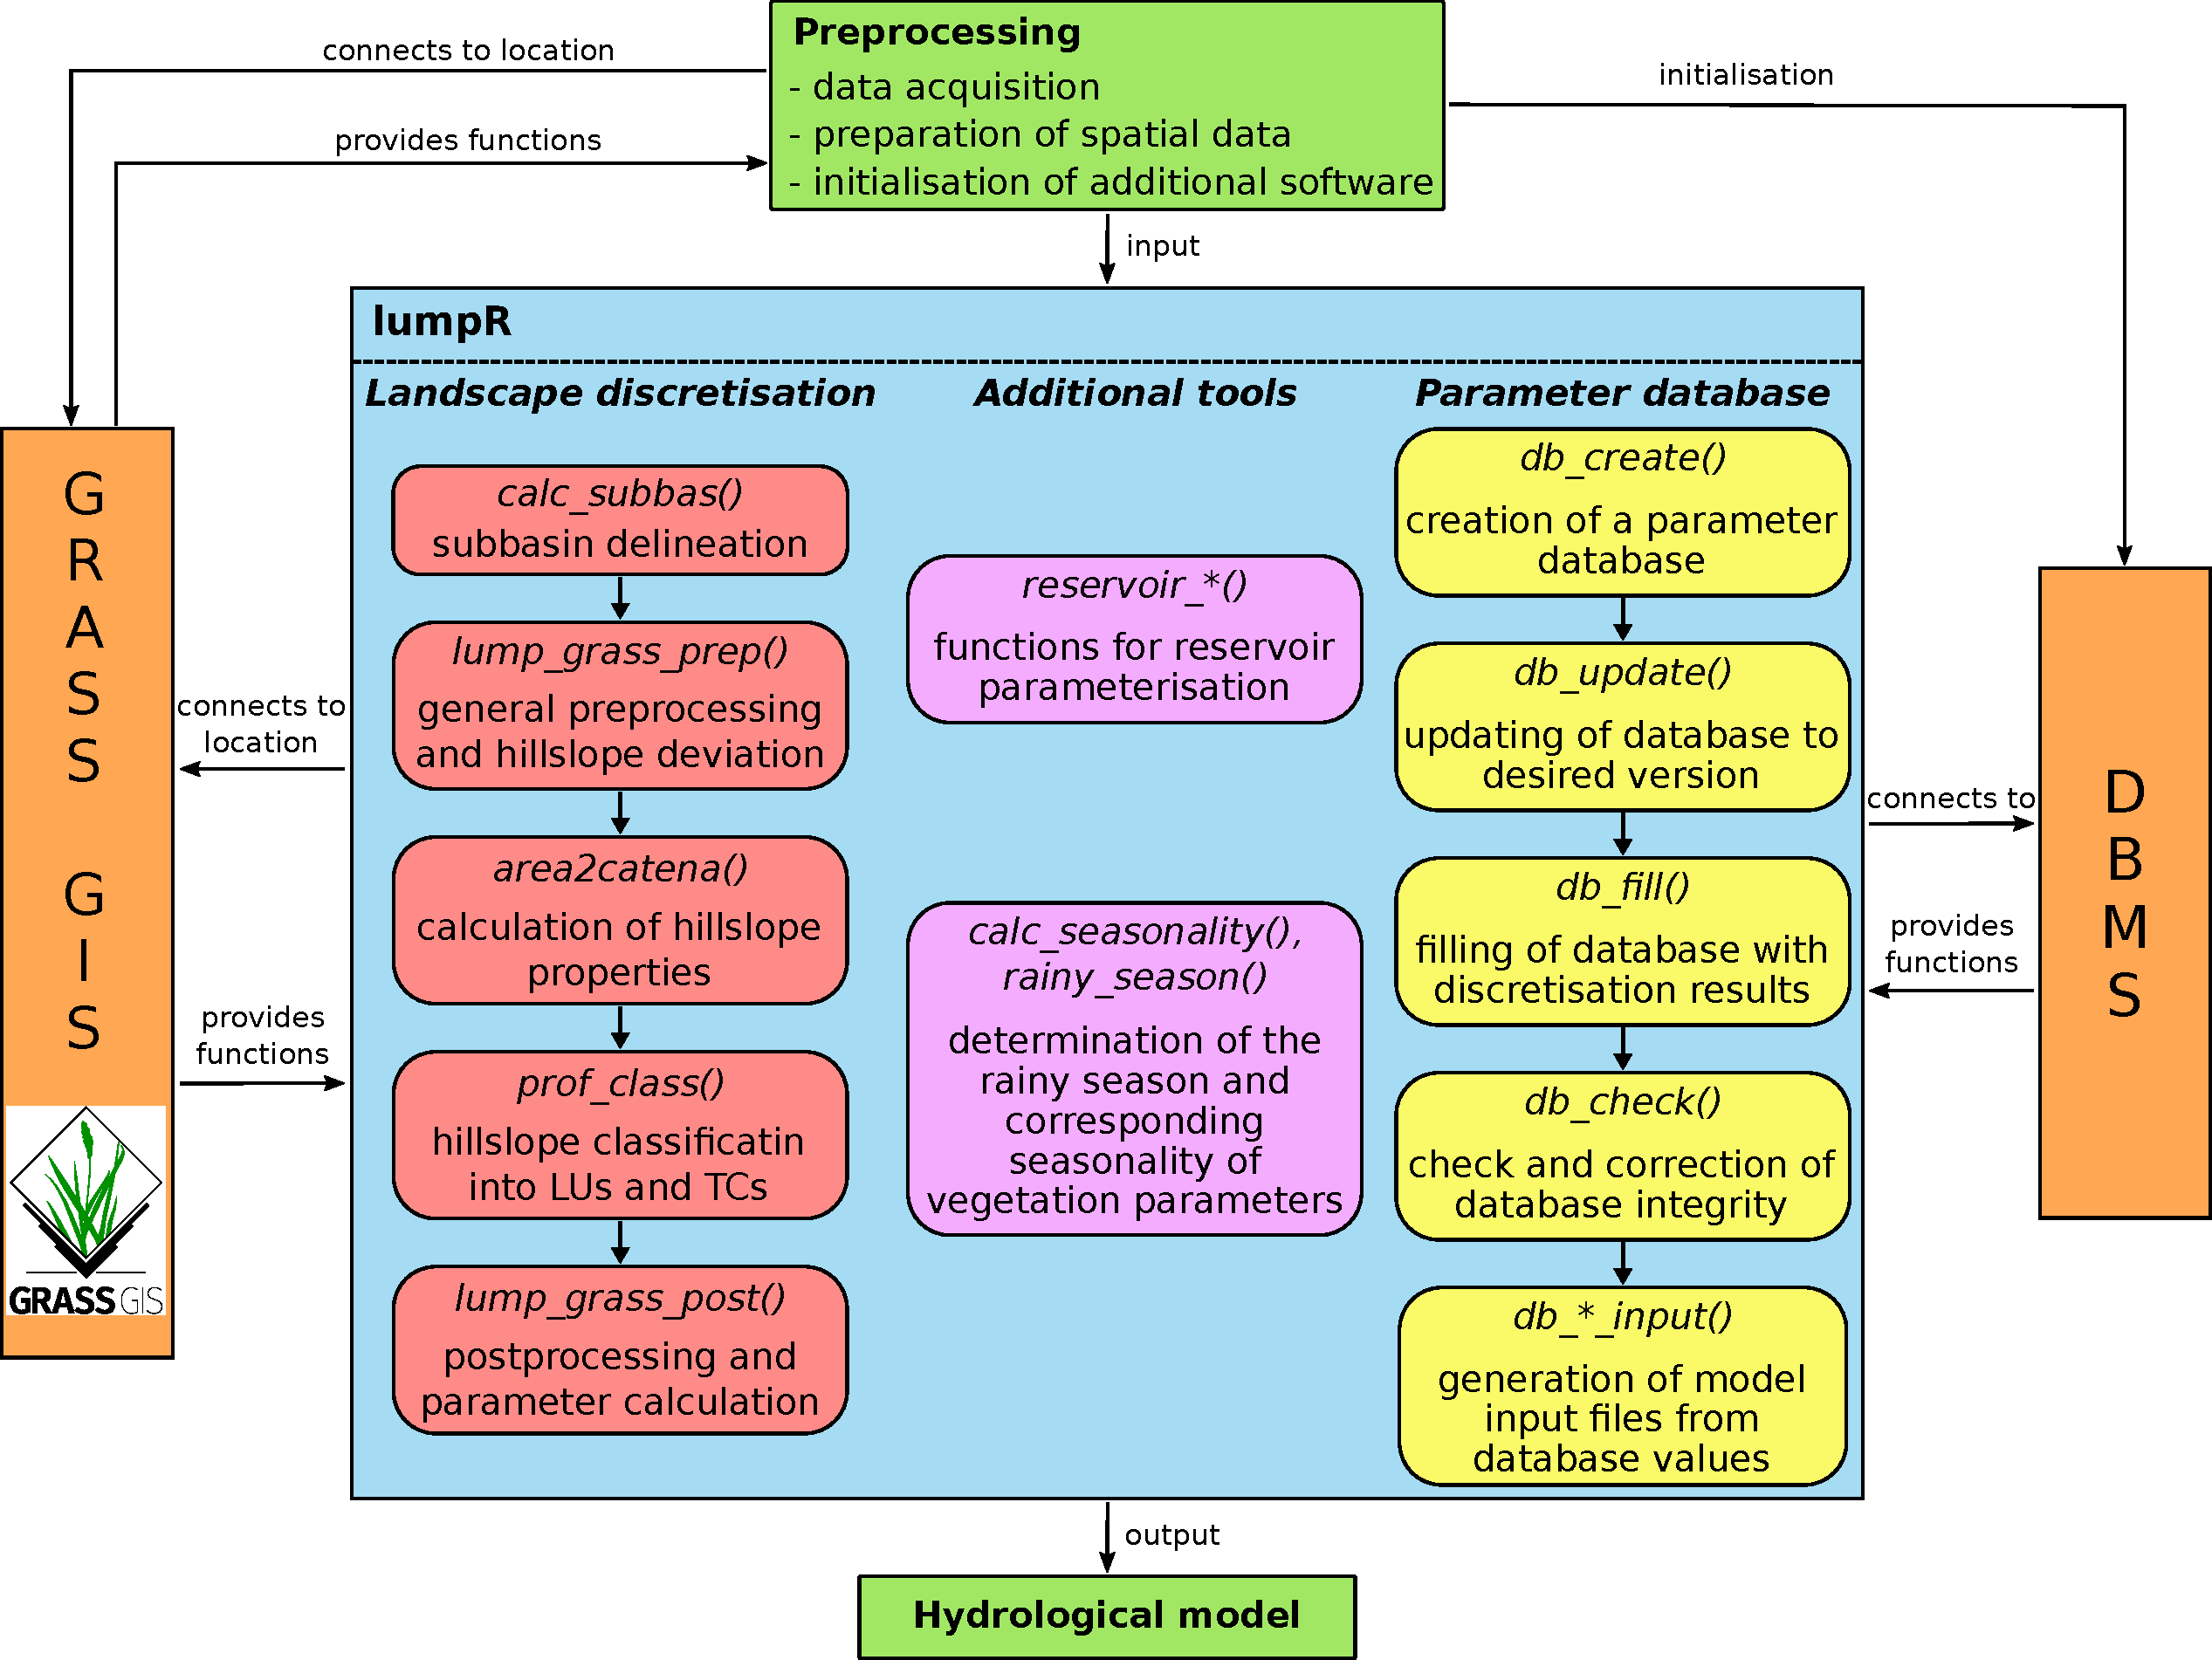
\includegraphics[width=\linewidth]{LUMP_scheme_coloured.pdf}
\caption{Schematic overview of the functionalities of the lumpR package. Shown are all available functions (\textit{in italics}) with a short explanation, interactions with external software, and flowcharts of typical workflows during application. Note that the acronym DBMS refers to \emph{DataBase Management System}.}
\label{fig:lumpr_scheme}
\end{figure*}


\subsection{Landscape discretisation}
\label{sec:landscape_discretisation}
After installing the package and all additionally needed software the user has to acquire and prepare all needed spatial data in a location in GRASS GIS.
Internally the package's functions connect to that location, use the given data for processing while partly employing GRASS functions, and finally stores the spatial output in the GRASS location and/or text files in a specified directory for immediate inspection after each function call.
As a first step in a new R session, before executing any of the package's function R has to be connected to the  GRASS location by the user as shown in the following example:

\begin{verbatim}
> library(lumpR)
> initGRASS(
>  gisBase = "/path/to/grass",
>  home = tempdir(),
>  location = "example_location",
>  mapset = "example_mapset",
>  gisDbase = "/path/to/grassdata")
\end{verbatim}

As is sketched in Fig. \ref{fig:lumpr_scheme} the process of landscape discretisation involves five functions that should be applied in the following order.
\emph{(i) calc\_subbas()} sub-divides the hydrological basin into subbasins using a given grid-based DEM.
Subbasin size can be influenced by the user by either giving a set of coordinates of drainage locations inferred beforehand or by specifying the parameter \verb|thresh_sub| being the minimum size of a subbasin in number of grid cells internally used by GRASS function r.watershed.
\emph{(ii) lump\_grass\_prep()} does several pre-processing steps needed for later use such as computing SVCs as simple overlay of soil and vegetation raster maps, inferring Horton stream order, and the calculation of hydrologically relevant landscape characteristics such as a flow direction, flow accumulation, relative elevation (i.e., elevations above next downstream river grid cell), and distance to next river grid cell put as raster maps into the initialised GRASS location.
Furthermore, the function infers EHAs based on the crucial size parameter \verb|eha_thres| that has to be given by the user.
\emph{(iii) area2catena()} takes generated data from step (ii) and supplemental raster maps of quantitative and/or qualitative variables to calculate a representative catena for every EHA characterised by horizontal and vertical length, shape (in terms of cumulated elevation along the hillslope), slope width (approximated by taking the number of grid cells at a profile point divided by the total number of grid cells representing the whole hillslope), and optional information from supplemental data.
The algorithm is based on the work of \citet{Cochrane2003} for the WEPP model.
\emph{(iv) prof\_class()} takes the representative catenas and classifies them into LUs.
In this step similar catenae are identified and lumped together based on the calculated properties employing an unsupervised K-means clustering method.
The user has to give a number of parameters affecting the importance of individual catena characteristics during the clustering.
Each LU is then further sub-divided into TCs, e.g., representing upper, middle, and downslope parts of the lumped catena.
The number of TCs to be generated for each LU is another input parameter.
For visual inspection of results the user has the option to let the functions generate plots during steps (iii) and (iv).
The employed algorithms for steps (iii) and (iv) are explained in more detail by \citet{Francke2008}.
Figure \ref{fig:lumpr_output}\TP{I still need to make an improved version of this figure. Suggestions?} gives an illustrative example for the outcome after applying steps (i) to (iv).

Finally, \emph{(v) lump\_grass\_post()} prepares subbasin and LU specific parameters as needed by the WASA model thereby employing rather simple relationships or typical standard values. The output of this function should therefore be carefully revised. See the function's documentation for more details.

\begin{figure}[t]
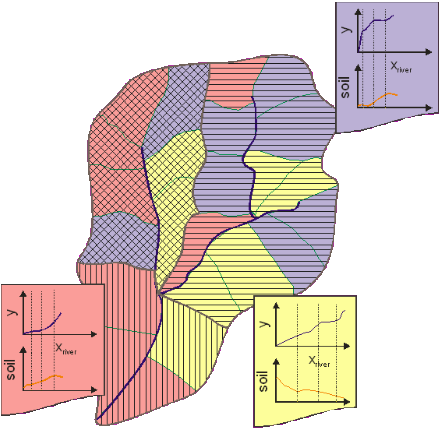
\includegraphics[width=\columnwidth]{lump_output.png}
\caption{Illustrative example of the outcome of steps (i) to (iv) of landscape discretisation. Shown is a hydrological basin sub-divided into subbasins (hatchures), EHAs (thin green lines), and LUs (colours). Average catena properties for the three LUs are exemplified by the coloured diagrams. TCs are indicated by vertical dashed lines in the diagrams.}
\label{fig:lumpr_output}
\end{figure}


\subsection{Additional tools}
In order to meet further capabilities of the WASA model functions \emph{reservoir\_*()} have been introduced.
They facilitate the pre-processing of reservoir-specific input files for the model using spatial reservoir data and pre-compiled parameterisations.
Additional function \emph{rainy\_season()} calculates start and end dates of the rainy season for every year based on a time series of daily precipitation values using a statistical approach described by \citet{Gerstengarbe1999}.
In WASA this information is needed as parameterisation of intra-annual variations of vegetation parameters.
\emph{calc\_seasonality()} takes output of the former function and information about seasonal variation of a vegetation parameter to calculate a daily time series of that parameter by linear interpolation of the parameter's node points depending on the current start and end dates of the rainy season for a specific year.
For more detailed information on vegetation parameterisation the reader may consult \citet{Guentner2002} and the function's documentations.
Although being rather specific to WASA the former functions may as well be of use for other models.


\subsection{Parameter database}
To store the results of landscape discretisation in a clearly arranged manner for readily generation of necessary model input files the package was enhanced by a set of database functions.
Guaranteeing platform independence and as much freedom of choice as possible to the user different frequently used \emph{DataBase Management Systems} (DBMS) are supported by lumpR currently including MS Access, MySQL / MariaDB, and SQLite.
As interface between R and the DBMS the \emph{Open DataBase Connectivity} (ODBC) in terms of the R package RODBC is employed.
To use a specific DMBS a number of pre-processing steps are necessary, such as installing required software and registering a new empty database as ODBC source, before applying the package's database functions.
For inexperienced users we prepared some general information on that topic in the Wiki of lumpR's web page (see section \ref{sec:code_availability}).
As for landscape discretisation the database functions might be applied in a defined order as indicated in Fig. \ref{fig:lumpr_scheme} and will be further explained in the following.

\emph{(i) db\_create()} creates the latest implemented version of all tables in the registered parameter database.
As the package underlies continuous further development which might also affect the parameter database \emph{(ii) db\_update()} was written to ensure compatibility between different database versions.
The user can specify to which version the current database shall be updated to include the latest changes in the database scheme to an existing database or to go back to an earlier version.
\emph{(iii) db\_fill()} takes text files produced as output of landscape discretisation and other pre-processing not included in the package (e.g., readily prepared soil and vegetation parameters) and fills the values into the respective tables of the parameter database.
\emph{(iv) db\_check()} performs a number of checks to identify and (if possible and desired) automatically resolve inconsistencies and/or missing information in the database.
These include filtering of tiny and insignificant areas (e.g., SVCs) to reduce computational overhead, checking that all TCs have a slope larger than zero, defining special areas for separate treatment (this currently includes SVCs marked as water or impervious), removing special areas marked was water, computing fractions of impervious surfaces at TC level, removing impervious surfaces, estimating a storage coefficient for groundwater delay (for a simple linear bucket approach of groundwater simulation) at LU level, deleting obsolete datasets (special area SVCs, LUs not in any subbasin, TCs not in any LU, and SVCs not in any TC), checking for completeness (all IDs in the \verb|*_contains_*| tables exist within the respective referenced tables), and computing the subbasin order from upstream (largest number) to downstream (one).
The user can decide which checks to perform, how to deal with inconsistencies, and define thresholds for certain checks. To keep an overview any changes to the database will be tracked in table \verb|meta_info|.

At any point during the processing the user can freely inspect and adjust the parameter database by means other than the functions provided by lumpR.
In the current version the package provides the function \emph{db\_wasa\_input()} to take the values of the parameter database and generate most of the generally necessary input files for WASA except for meteorological forcing and files related to sediment routing and reservoirs.
However, the user may as well export the values needed and compile the input files for any other model that makes use of the values assembled in the parameter database.
Furthermore, it is a straightforward task to extent the package and include export functions for other models if requested.




\section{Example application and sensitivity analysis}
\label{sec:methods}

\subsection{Study site}
\label{sec:study_site}
To demonstrate the functionalities of lumpR the Bengu\^e catchment was selected (Fig. \ref{fig:catchment}\TP{I guess this figure could still be improved as well. And it needs a north arrow.}).
It is part of the upper Jaguaribe river catchment in the northeast of Brazil within the federal state of Cear\'a.
The area has been investigated in a number of studies, in many cases employing the WASA model, and was thus selected to ensure the ability of the model for the catchment \citep{Medeiros2010,Krol2011,deAraujo2013,Bronstert2014,Medeiros2014a,Medeiros2014b,Figueiredo2016}. \TP{Other or more studies to be cited?}

\begin{figure*}[t]
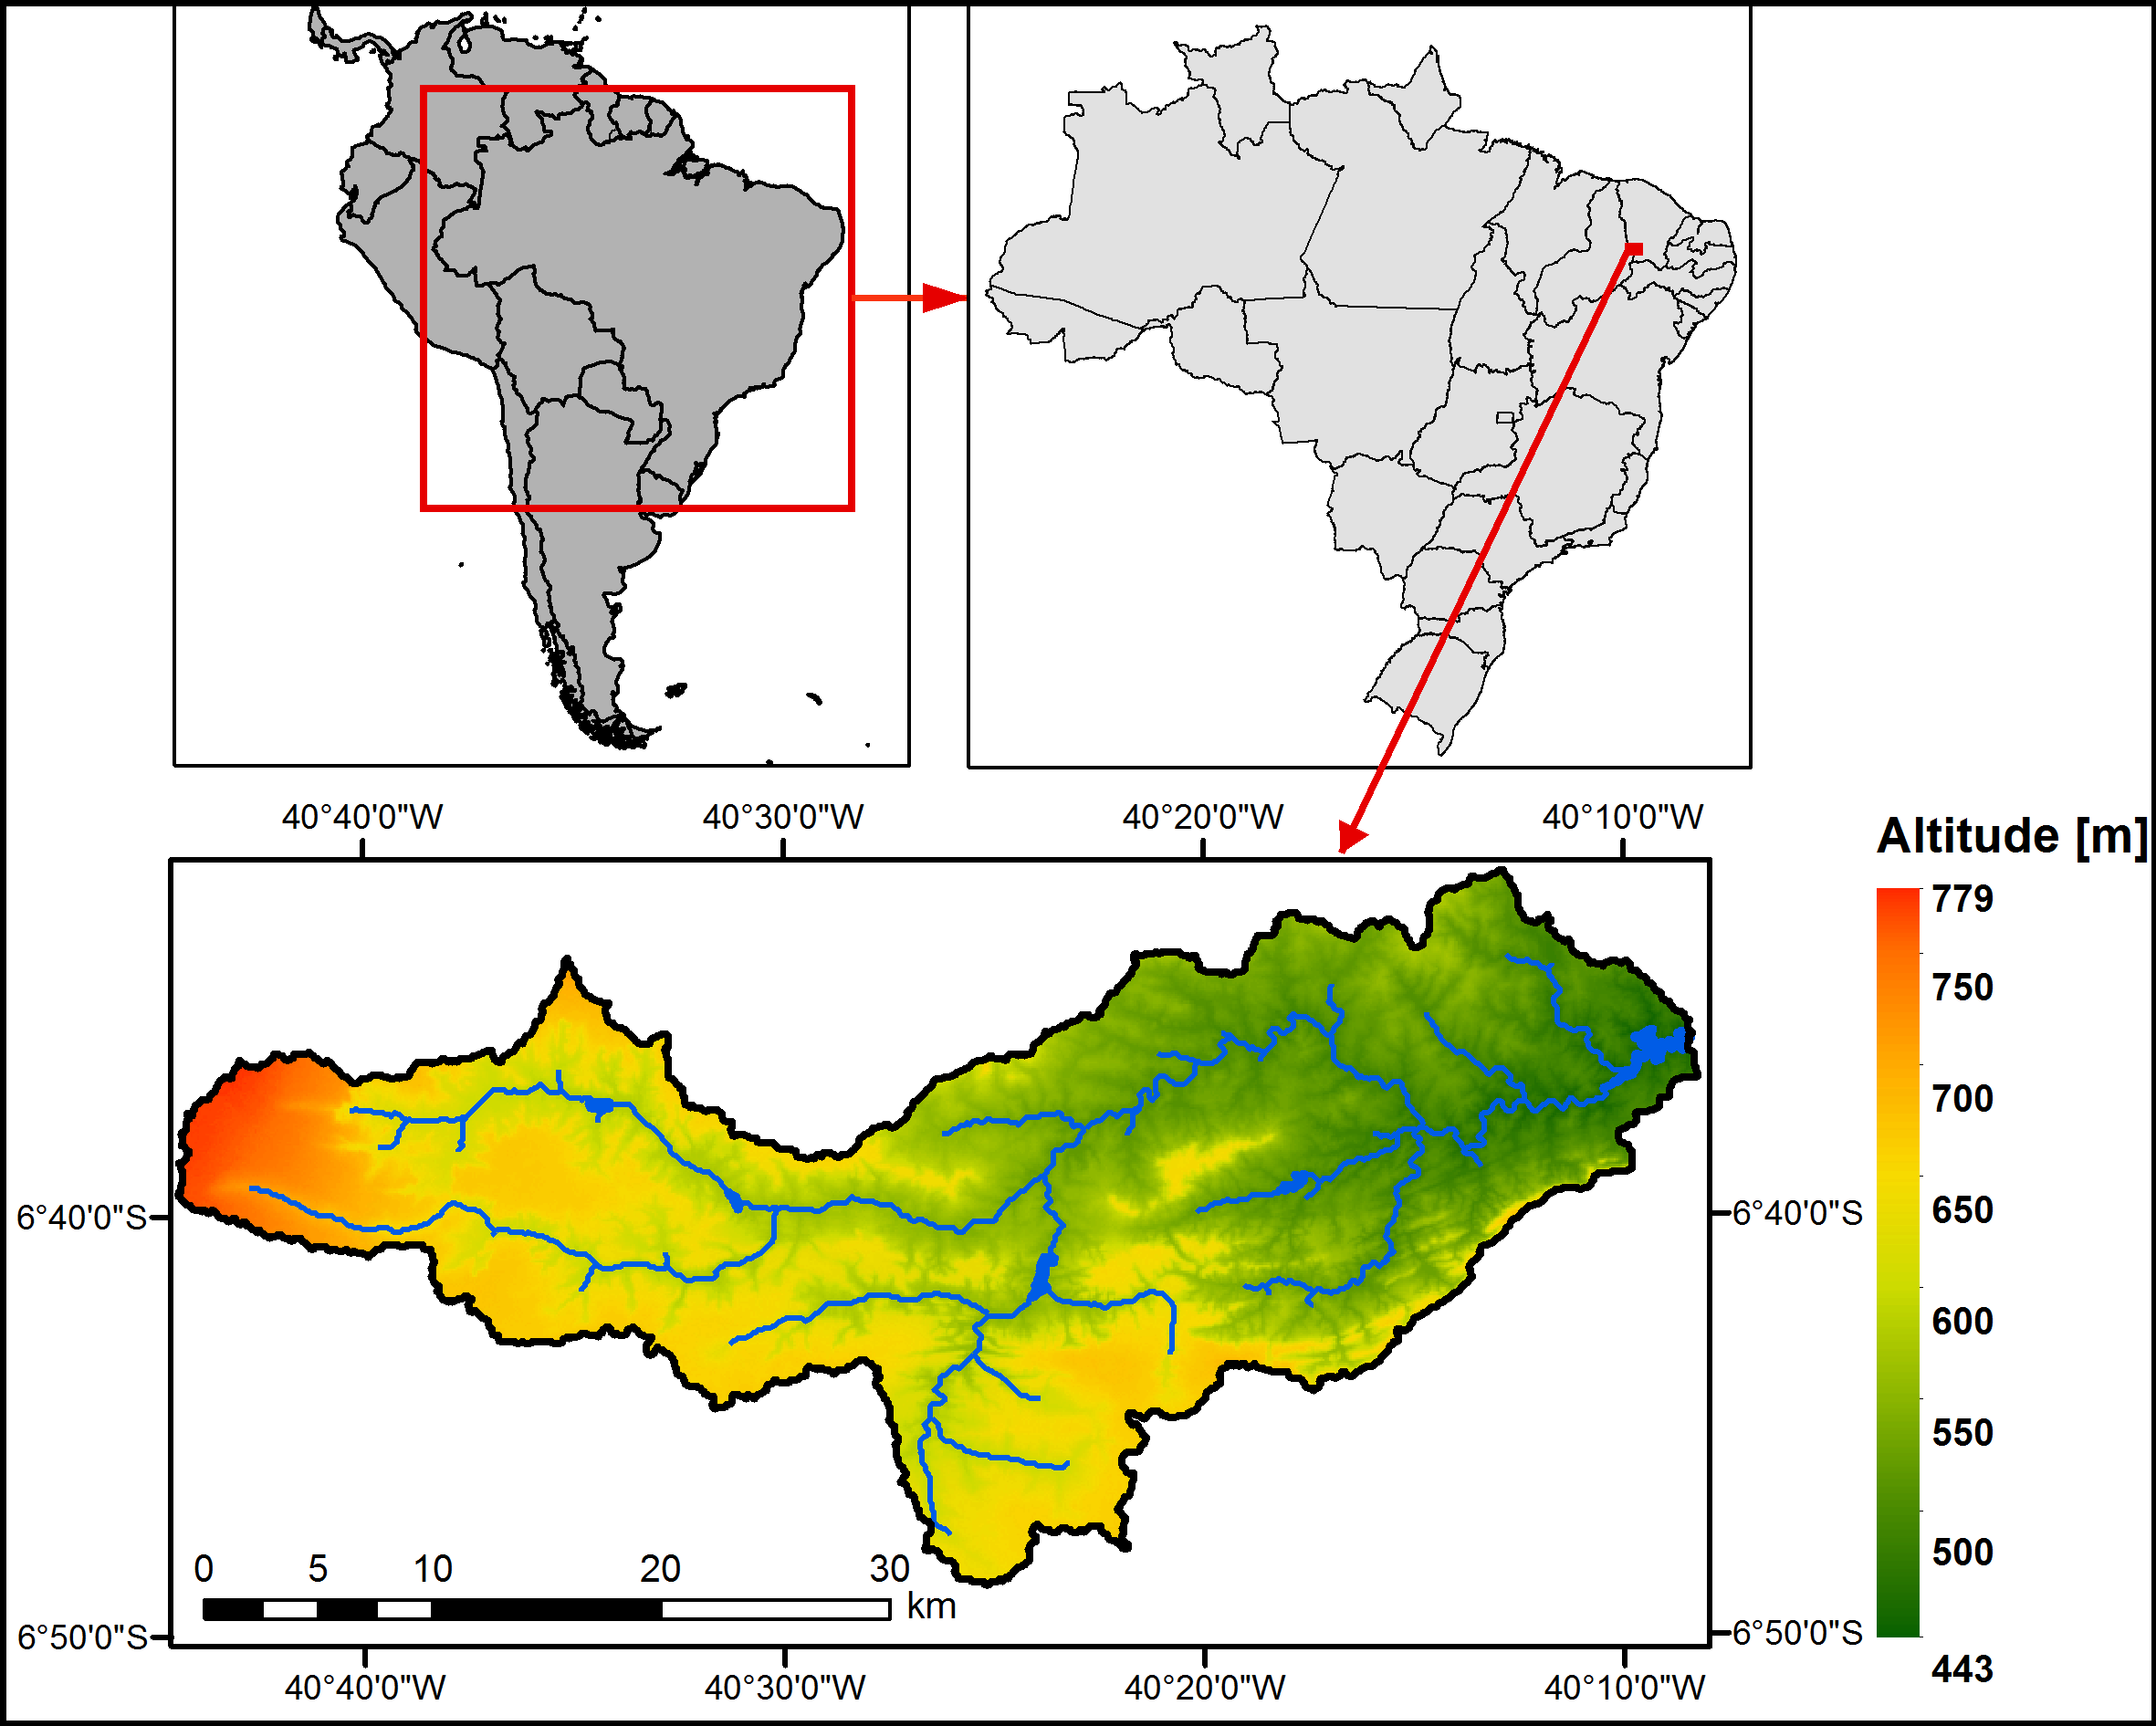
\includegraphics[width=\linewidth]{overview_bengue_2.png}
\caption{Overview over the Bengu\^e catchment (lower panel) and location within Brazil (upper right) and South America (upper left), respectively.}
\label{fig:catchment}
\end{figure*}

The Bengu\^e catchment drains an area of about 926 \unit{km^2}.
At the outlet the ephemeral Umbuzeiro river is constrained by a reservoir built in 2000 with a storage capacity of 19.6 million \unit{m^3} to enhance water supply and reliability in the region.
As the area is located within the "drought polygon" of Brazil annual average precipitation is low with about 600 \unit{mm} in comparison to a potential evapotranspiration of more than 2000 \unit{mm}.
The mean annual temperature is 25 \unit{\degree C} with little variation.
Climate is further characterised by a strong intra-annual variation of precipitation leading to distinct rainy (January to May with more than 80 \% of annual rainfall) and dry seasons.
Rainfall is mostly convective and concentrated in only a few events a year with high intensity.
Inter-annual variation of precipitation, however, is also high causing recurrent droughts which in cases may last over several consecutive years.
The dominant natural vegetation is Caatinga consisting of deciduous bushland with xerophytic species ranging from dense dry forests to almost desert-like sites.
The population density is low (6.4 inhabitants per \unit{km^2}) with rural lifestyle.
Parts of the area are used for small-scale farming including cattle-breeding and growing of maize and beans in particular.
The environment is further characterised by mainly sedimentary plateaus in the southern and western parts of the study site with steep terrain and deep (> 1 m) permeable soils, predominantly Latosols.
In the North and East crystalline bedrock is prevailing with shallow Luvisols (< 1 m) causing high runoff coefficients.
In alluvial zones Planosols are dominant.


\subsection{WASA model}
\label{sec:wasa}
The WASA model is used to study the effects of different landscape discretisations realised with lumpR on simulated streamflow dynamics.
The model was first introduced by and is described in detail within \citet{Guentner2002}.
It has been frequently employed in semi-arid areas such as northeastern Brazil (including the Bengu\^e catchment; for references see section \ref{sec:study_site}), India \citep{Jackisch2014} and Spain \citep{Mueller2009,Mueller2010,Bronstert2014}.
For information on model availability the reader is referred to section \ref{sec:code_availability}.

WASA is a deterministic, process-based, semi-distributed, time-continuous hydrological model.
It is dedicated to natural semi-arid environments.
The model incorporates the Shuttleworth-Wallace approach for evapotranspiration calculation over sparsely vegetated surfaces and an infiltration approach based on Green-Ampt accounting for Horton-type infiltration.
Via the complex hierarchical spatial disaggregation scheme (cf. section \ref{sec:review_approaches}) lateral re-distribution processes as well as ex- and re-infiltration along a hillslope are considered while the model can still be applied over large scales (up to the order of magnitude of 100,000 \unit{km^2}).
Large strategic reservoirs can be represented in an explicit manner while smaller ones are treated as lumped lakes of different size classes to efficiently account for water retention of many small reservoirs in a study region.
The model has been subsequently expanded to account for sediment dynamics with several optional USLE-based approaches \citep{Mueller2010}, whereas it was henceforth called WASA-SED.
As in this study no erosional processes are considered the model shall herein furthermore termed WASA.


\subsection{Data and model setup}
Meteorological data in daily resolution to drive WASA, in particular precipitation, air temperature (obtained by minimum and maximum temperatures by simple averaging), relative humidity, and incoming short-wave radiation, have been derived from the dataset described by \citet{Xavier2016}.
The gridded dataset is based on station information that have been checked, corrected, and interpolated to a grid with 0.25\unit{\degree} x 0.25\unit{\degree} resolution.
Extraterrestrial radiation as a further driver that has been calculated from astronomical relationships employing the R package \emph{sirad}.
Meteorological data have been interpolated to the locations of subbasin centroids using an inverse-distance weighting approach  by employing the R package \emph{geostat}.\footnote{This package is not on CRAN but available via the ECHSE tools library from \url{https://github.com/echse/echse_tools}.}

The basis of terrain analyses was the 90\unit{m} x 90\unit{m} grid-based SRTM DEM.
As pre-processing step the raw raster has been sink-filled employing the GRASS function \emph{r.terraflow}.
Soil information have been derived from the database of \citet{Jacomine1973}.
The parameters needed by WASA have been inferred by pedo-transfer functions based on soil texture information using the R packages \emph{soilwaterfun} and \emph{soilwaterptf} available via \url{http://soilwater.r-forge.r-project.org/}.
Vegetation parameters for the types occurring within the study area have been elaborated during the development of WASA \citep{Guentner2002} and have been adopted for this study.
An updated shapefile of landcover distribution could be obtained from the Brazilian ministry for the environment and the land cover classes have been reclassified to those used in \citep{Guentner2002}.
Data on reservoirs and the geology of the area have been collected and processed within the SESAM project, see \url{http://www.uni-potsdam.de/sesam}.

It should be stressed that WASA has been initialised by using only independent observational data.
No calibration of any model parameters has been done as a comparison with observational data shall not be part of this study. 
As has been mentioned, however, the model has been used in and proved its ability for the catchment (see references given in section \ref{sec:study_site}).


\subsection{Sensitivity analysis of user decisions}
During the process of model initialisation and landscape discretisation a user commonly has to make a number of often subjective decisions.
These are directly influencing the complexity of discretisation and thereby affecting computational efforts and possibly model results.
Due to the complexity of the software, the diversity of links, and potentially non-linear relationships the effects of these user decisions shall be analysed by conducting a number of numerical experiments.
User decisions are thereby treated as parameters within a model sensitivity analysis.
Each experiment within the analysis stands for a specific realisation of parameters in turn referring to a particular landscape discretisation setup used to drive WASA.


\subsubsection{Experimental setup}

\begin{table}[t]
\caption{User decisions affecting landscape discretisation complexity and their realisations used for sensitivity analysis.}
\begin{tabularx}{\columnwidth}{L{.25}L{.45}C{.3}}
\tophline
Identifier & Meaning & Realisations\\
\middlehline
SUB\_thresh & Minimum size of subbasins in number of grid cells & 1000, 2000, 5000, 10000, 30000\\
EHA\_thresh & Minimum size of EHAs in number of grid cells & 25, 50, 100, 200, 500, 750, 1000\\
LU\_no & Maximum number of LUs to be classified & 5, 10, 20, 50, 75, 100, 150, 200, 250, 300\\
LU\_atts & Number of attributes to be considered during LU classification & 1...7 \\
TC\_no & Number of TCs to be deviated for every LU & 1...5\\
\bottomhline
\end{tabularx}
%\belowtable{} % Table Footnotes
\label{tab:pars}
\end{table}

For landscape discretisation using lumpR five parameters reflecting the most important user decisions have been identified and are summarised in Tab. \ref{tab:pars}.
Their presented realisations are based on a priori knowledge and should span a reasonable value range at the one hand and,  at the other hand, result in as much as possible variation in generated spatial units.
Therefore, for some parameters such as \verb!SUB_thresh!, also non-uniform distributions of realisations have been taken into account.
All in all it should be noted that a general statement on which parameter realisation is the most plausible and suitable one can hardly be given as the choices are strongly case study specific and partly also depend on available data.
What follows is a reasoning on selected parameter realisations for the experiments that can be used as guidelines for lumpR applications.

\verb!SUB_thresh! and \verb!EHA_thresh! are size thresholds internally directed to the GRASS function \emph{r.watershed} affecting the size and thereby the number of delineated subbasins and EHAs, respectively.
As their realisations are given in number of grid cells their choice depends on the resolution of the GRASS location (herein the SRTM DEM resolution of 90\unit{m} x 90\unit{m} was used), and catchment size.
\verb!LU_no! and \verb!LU_atts! control the process of clustering EHAs into LUs.
The maximum possible value for \verb!LU_atts! depends on the available information that can be used for classification.
This generally includes the shape of EHAs, their horizontal and vertical extension, and a proxy for hillslope width which are all inferred from a DEM.
Further supplemental attributes can be added which in this study included raster maps of soil types, land cover, geology, and SVCs that resulted in a total of seven attributes.
For the experiments different realisations of \verb!LU_atts! shall reflect a differing degree of information available for the deviation of LUs.
Which of the aforementioned attributes are used for a certain experiment is sampled randomly.
Each attribute then gets assigned a factor meaning that for every attribute that many LUs shall be deviated.
\verb!LU_no! defines the maximum number of LUs to be generated.
Hence, due to the multiplicative nature of the number of LUs to be generated, a factorisation approach is employed to derive the factors for each attribute.
Herein, one of the sampled attributes is randomly selected and its factor increased by one.
This procedure is repeated until the product of factors, i.e., the actual number of LUs, is greater than or equal to \verb!LU_no!.
Finally, \verb!TC_no! is the number of TCs that will be delineated for every LU.
The minimum number of one would effectively result in treating a single LU without further sub-discretisation into TCs.
A number larger than five, although this decision is somewhat subjective, seemed rather futile due to increasing computational burden and being harder to interpret in a geomorphologically meaningful way.

For the sensitivity analysis all possible combinations of parameter realisations have been employed which resulted in a total of 12,250 experiments.
This comprises varying complexities within all spatial levels and different degrees of data availability.
All discretisations have been realised using lumpR as explained in section \ref{sec:landscape_discretisation} employing always the same framework and varying only the aforementioned parameters.
Finally, WASA has been run with each realisation over a 13 year period whereas the first five years were considered as warm-up and thus have been excluded from the analysis.

\subsubsection{Scalar model output}

\begin{table*}[t]
\caption{Streamflow indices used as scalar response functions for sensitivity analysis.}
\begin{tabularx}{\textwidth}{L{.1}L{.25}L{.5}L{.15}}
\tophline
Symbol & Index & Calculation & Unit\\
\middlehline
$RR$ & Runoff ratio & Sum of daily streamflow values divided by sum of daily precipitation over the whole period of analysis multiplied by 100 & \unit{\%}\\
$P_{flow}$ & Probability for significant streamflow & Number of days with significant$^1$ streamflow divided by total number of values multiplied by 100 & \unit{\%}\\
$Q_{avmax}$ & Average annual maximum flow & Average over all annual maximum streamflow values & \unit{m^3 s^{-1}}\\
$SFDC$ & Slope of flow duration curve & Average slope of the flow duration curve for significant$^1$ medium ranged$^2$ streamflow values & dimensionless\\
$f_{low}$ & Frequency of low flows & Average number of insignificant$^1$ flow events$^3$ per year & \unit{year^{-1}}\\
$f_{high}$ & Frequency of high flows & Average number of high flow$^4$ events$^3$ per year & \unit{year^{-1}}\\
$RC_{rise}$ & Rate of change during rise & Average rate of change of the rising limbs of high flow$^4$ events$^3$ & \unit{m^3 s^{-1} day^{-1}}\\
$RC_{fall}$ & Rate of change during fall & Average rate of change of the falling limbs of high flow$^4$ events$^3$ & \unit{m^3 s^{-1} day^{-1}}\\
\bottomhline
\end{tabularx}
\belowtable{(1) (In-) significant streamflow defined as those values (less than or equal to) larger than 0.01 \unit{m^3 s^{-1}}.\\
(2) Values between the 33 \unit{\%} and 66 \unit{\%} percentiles.\\
(3) An event is defined as a period of consecutive days a certain condition is fulfilled.\\
(4) High flows are those values being larger than a flow threshold which is herein defined as the 90 \unit{\%} percentile of all significant$^1$ flow values from all 12,250 model realisations during the analysis period.}
\label{tab:indices}
\end{table*}

The target variable of the analysis is the time series of simulated daily river contributions to the Bengu\^e reservoir located at the catchment outlet.
However, for conduction of sensitivity analyses a scalar target function is generally needed.
As it is impossible to summarise all important characteristics of a streamflow time series in a single scalar value it was decided to employ a whole set of indices and perform the sensitivity analysis for each index separately.
The indices are presented and described in Tab. \ref{tab:indices}.
As it can be seen the set of indices describes different aspects of streamflow behaviour ranging from the magnitude of flow ($RR$, $P_{flow}$, $Q_{avmax}$) over flow regime ($SFDC$)\footnote{High values stand for a more variable whereas low values represent a more damped flow regime \citep{Sawicz2011}.} to frequency ($f_{low}$, $f_{high}$) and runoff concentration time ($RC_{rise}$, $RC_{fall}$). 

\subsubsection{Analysis method}

There exists a large number of approaches for sensitivity analysis.
The selection basically depends on the objective of the study, the nature and complexity of the model, its parameters and outputs, and available computing resources.
For the latest review of methods and guidelines for practical application in environmental studies see \citet{Pianosi2016a}.

The goals of this analysis were, first, a \emph{ranking} of the described descritisation parameters (sometimes also referred to as \emph{priorisation}) and, second, the identification of those parameters with negligible influence on the respective streamflow index (also referred to as \emph{screening} or \emph{fixing}).
As has been described above, model parameters were sampled over their entire (a priori as meaningful defined) value ranges and varied at the same time within individual runs which leads to a \emph{global} sensitivity analysis with \emph{all-at-a-time} sampling.
Based on these considerations \citet{Pianosi2016a} suggest a variance- or density-based approach.
The former is based on the calculation of sensitivity indices based on the variance of the response function.
This, however, requires the assumption that the variance is a good proxy for describing the variation of the value range.
For multi-modal or highly-skewed distributions this cannot be guaranteed.
In such a case \citet{Pianosi2016a} recommend density-based methods.
Rather than the variance alone this family of sensitivity analyses considers the probability density function of the response surface.
We decided on using the recently introduced PAWN method by \citet{Pianosi2015} as this density-based method can cope with skewed distributions and is relatively easy and straightforward to implement.

PAWN uses empirical approximations of the unconditional cumulative distribution function $F_{y_i}(y_i)$, with $y_i$ being one of the streamflow indices selected as scalar response functions over all 12,250 realisations, and the conditional cumulative distribution functions $F_{y_i|p_j}(y_i)$ where a certain parameter $p_j$ is fixed at a specific value.
The PAWN index $T_j$ as a sensitivity measure can then be calculated for each parameter employing a numerical approximation of the Kolmogorov-Smirnov statistic $KS$ following

\begin{equation}
	KS(p_j) = \max_{y_i} \Bigl| F_{y_i}(y_i) - F_{y_i|p_j}(y_i) \Bigr|
\end{equation}
and
\begin{equation}
	T_j = \underset{p_j}{\mathrm{median}} \Bigl[ KS(p_j) \Bigr]
\end{equation}

$T_j$ varies between 0 and 1.
It was used to rank the parameters in which lower values of $T_j$ identify the less influential ones.
For parameter screening the two-sample Kolmogorov-Smirnov test was employed.
It calculates a critical value $KS_{crit}$ below or equal to which a parameter can be judged insignificant as its conditional cumulative distribution function differs significantly from the unconditional one at a certain confidence level $\alpha$:

\begin{equation}
	KS_{crit} = c(\alpha) \sqrt{\frac{n+m}{nm}}
\end{equation}
with $n$ and $m$ being the number of samples to estimate $F_{y_i}(y_i)$ and $F_{y_i|p_j}(y_i)$, respectively, and $c(\alpha)$ being a literature value.
Herein we set $\alpha = 0.05$ and thus $c(\alpha) = 1.36$.


\subsection{Results}
\label{sec:results}

\begin{figure*}[t]
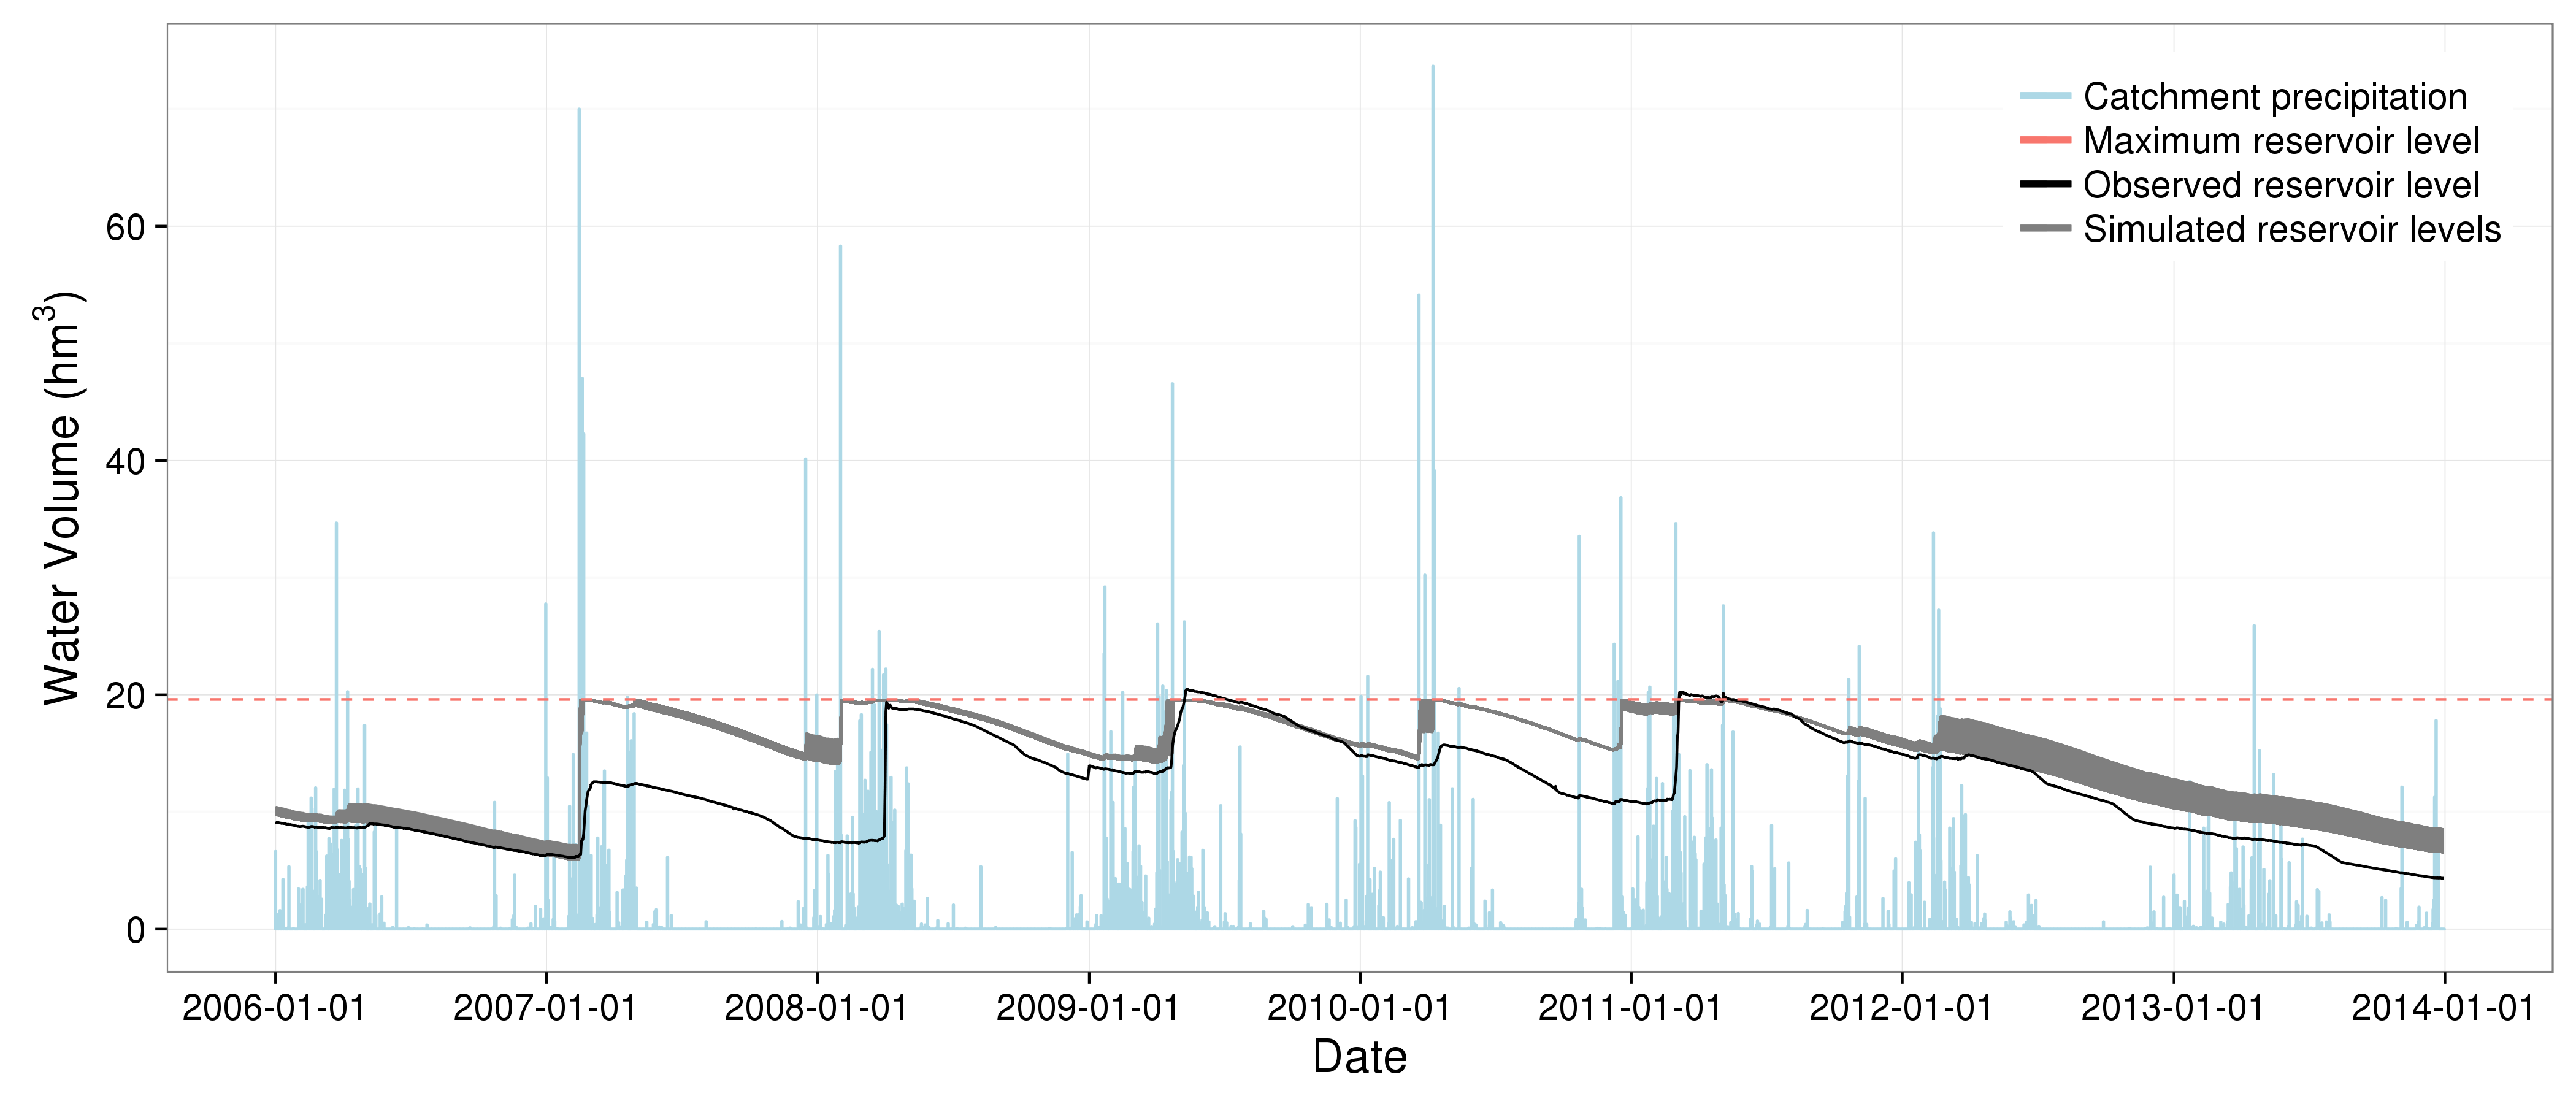
\includegraphics[width=\linewidth]{../analysis/comparison_results/Bengue_resvol_overview.png}
\caption{Time series plot of daily resolution of simulated (all 12,250 experiment runs) and observed Bengu\^e reservoir volume and areal precipitation.}
\label{fig:resvol}
\end{figure*}

Figure \ref{fig:resvol} provides and overview over the daily model results in comparison to observations for the Bengu\^e reservoir at the catchment outlet together with the catchment's areal precipitation used to drive the model.
Absolute deviations of uncalibrated model runs from observations are large whereas qualitative behaviour is matched well.
However, in some years (2008 and 2011) the model simulates reservoir filling within the rainy season much earlier than observed.
For the simulations, a rainfall volume of at least about 35 \unit{hm^3} seems to be necessary to produce significant reservoir inflow.
Simulated reservoir depletion is often slower than it can be observed.
Overall it should be noted that variability within the experiments is rather small whereas deviations seem to be originated from differing sensitivities of streamflow to a certain rainfall input.

\begin{figure*}[t]
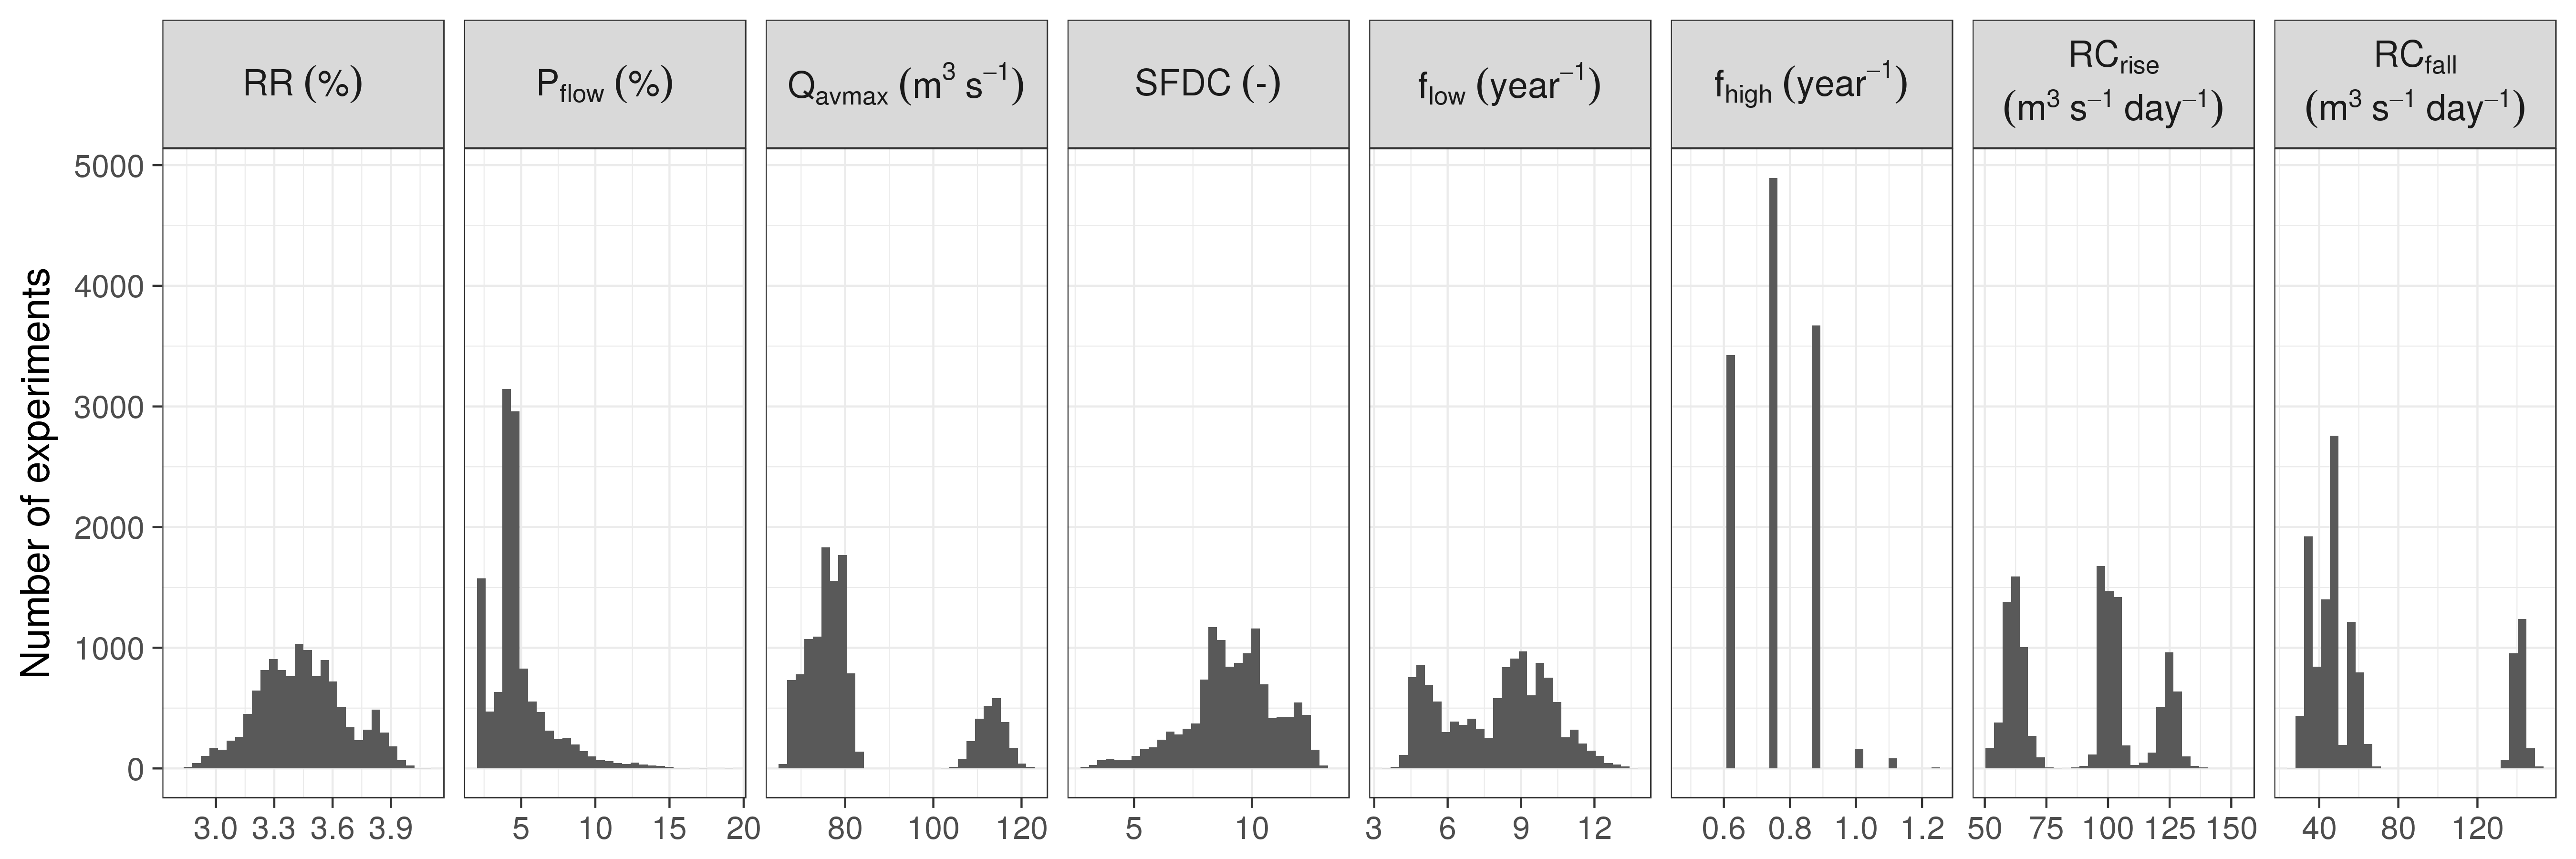
\includegraphics[width=\linewidth]{../analysis/sensitivity/hist_hydIndices_overview.png}
\caption{Histograms showing the value distributions of streamflow indices over the 12,250 experiments.}
\label{fig:hydIndices}
\end{figure*}

Figure \ref{fig:hydIndices} gives an overview of the streamflow index value distributions from the 12,250 experiments.
It can be seen that some indices, namely $Q_{avmax}$, $f_{high}$, $RC_{rise}$, and $RC_{fall}$, show distinct multi-modal value distributions.
Distributions for the other indices are slightly bi-modal ($f_{low}$) or skewed ($P_{flow}$ and $SFDC$) with $RR$ as the only index being more or less normal distributed.
In general, the runoff coefficient $RR$ is consistently low ranging between 3 \unit{\%} and 4 \unit{\%} and streamflow can be characterised as ephemeral due to a low probability of days showing significant streamflow ($P_{flow}$ about 5 \unit{\%} for most of the experiments).
Contrary to low flow periods, high flow events do rarely occur whereas the variability between experiments is high ($f_{low}$ and $f_{high}$, respectively).
Peak flows ($Q_{avmax}$) as well as runoff concentrations (characterised by $RC_{rise}$ and $RC_{fall}$) vary considerably between experiments also exhibiting multi-modal distributions.

\begin{figure*}[t]
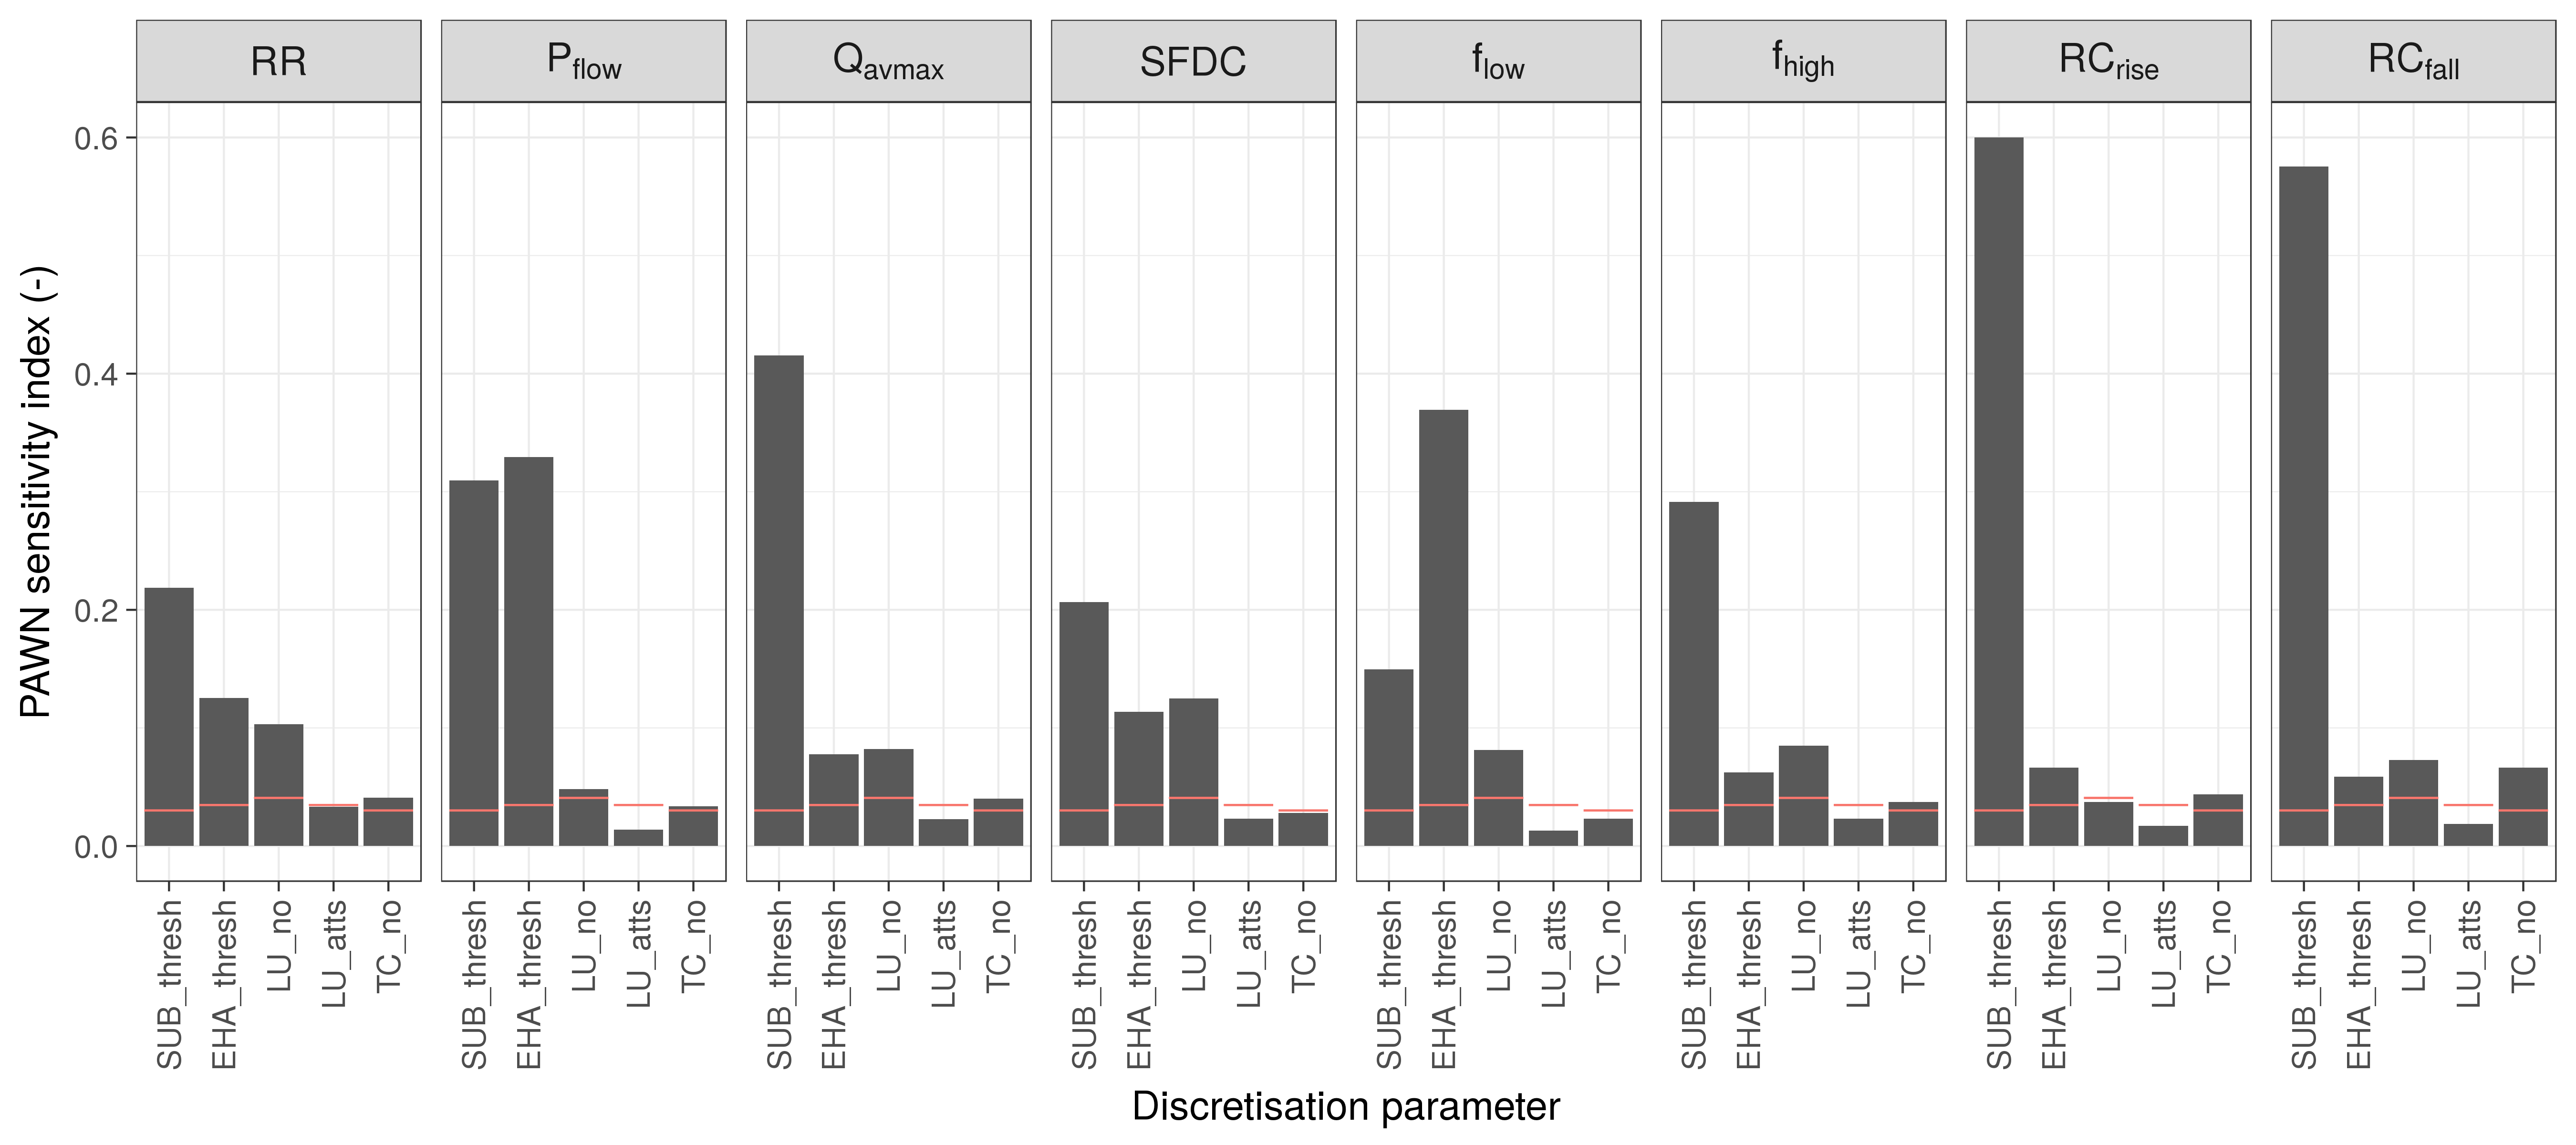
\includegraphics[width=\linewidth]{../analysis/sensitivity/sensitivity_PAWN_bars.png}
\caption{Barplots of PAWN sensitivity indices for each streamflow index and landscape discretisation parameter. Red lines indicate critical Kolmogorov-Smirnov values ($KS_{crit}$), i.e., parameters for which the PAWN index is less than or equal to this value can be regarded as insignificant for a specific streamflow index.}
\label{fig:PAWNbars}
\end{figure*}

Screening and ranking of landscape discretisation parameters is exhibited with Fig. \ref{fig:PAWNbars}.
The size of subbasins (\verb!SUB_thresh!) is the most influential parameter for all indices except for those being related to low flow characterisation ($f_{low}$ and $P_{flow}$) which are dominated by the size of EHAs (\verb!EHA_thresh!).
The number of LUs (\verb!LU_no!) can be regarded as the third important parameter being especially of relevance for high flow related indices ($f_{high}$ and $Q_{avmax}$) and, to some extent, flow regime ($SFDC$) and runoff concentration ($RC_{fall}$).
The least important parameters are the number of TCs (\verb!TC_no!), except for runoff concentration ($RC_{rise}$ and $RC_{fall}$), and the number of attributes considered for LU classification (\verb!LU_atts!) which is insignificant for all streamflow indices.

\begin{figure*}[t]
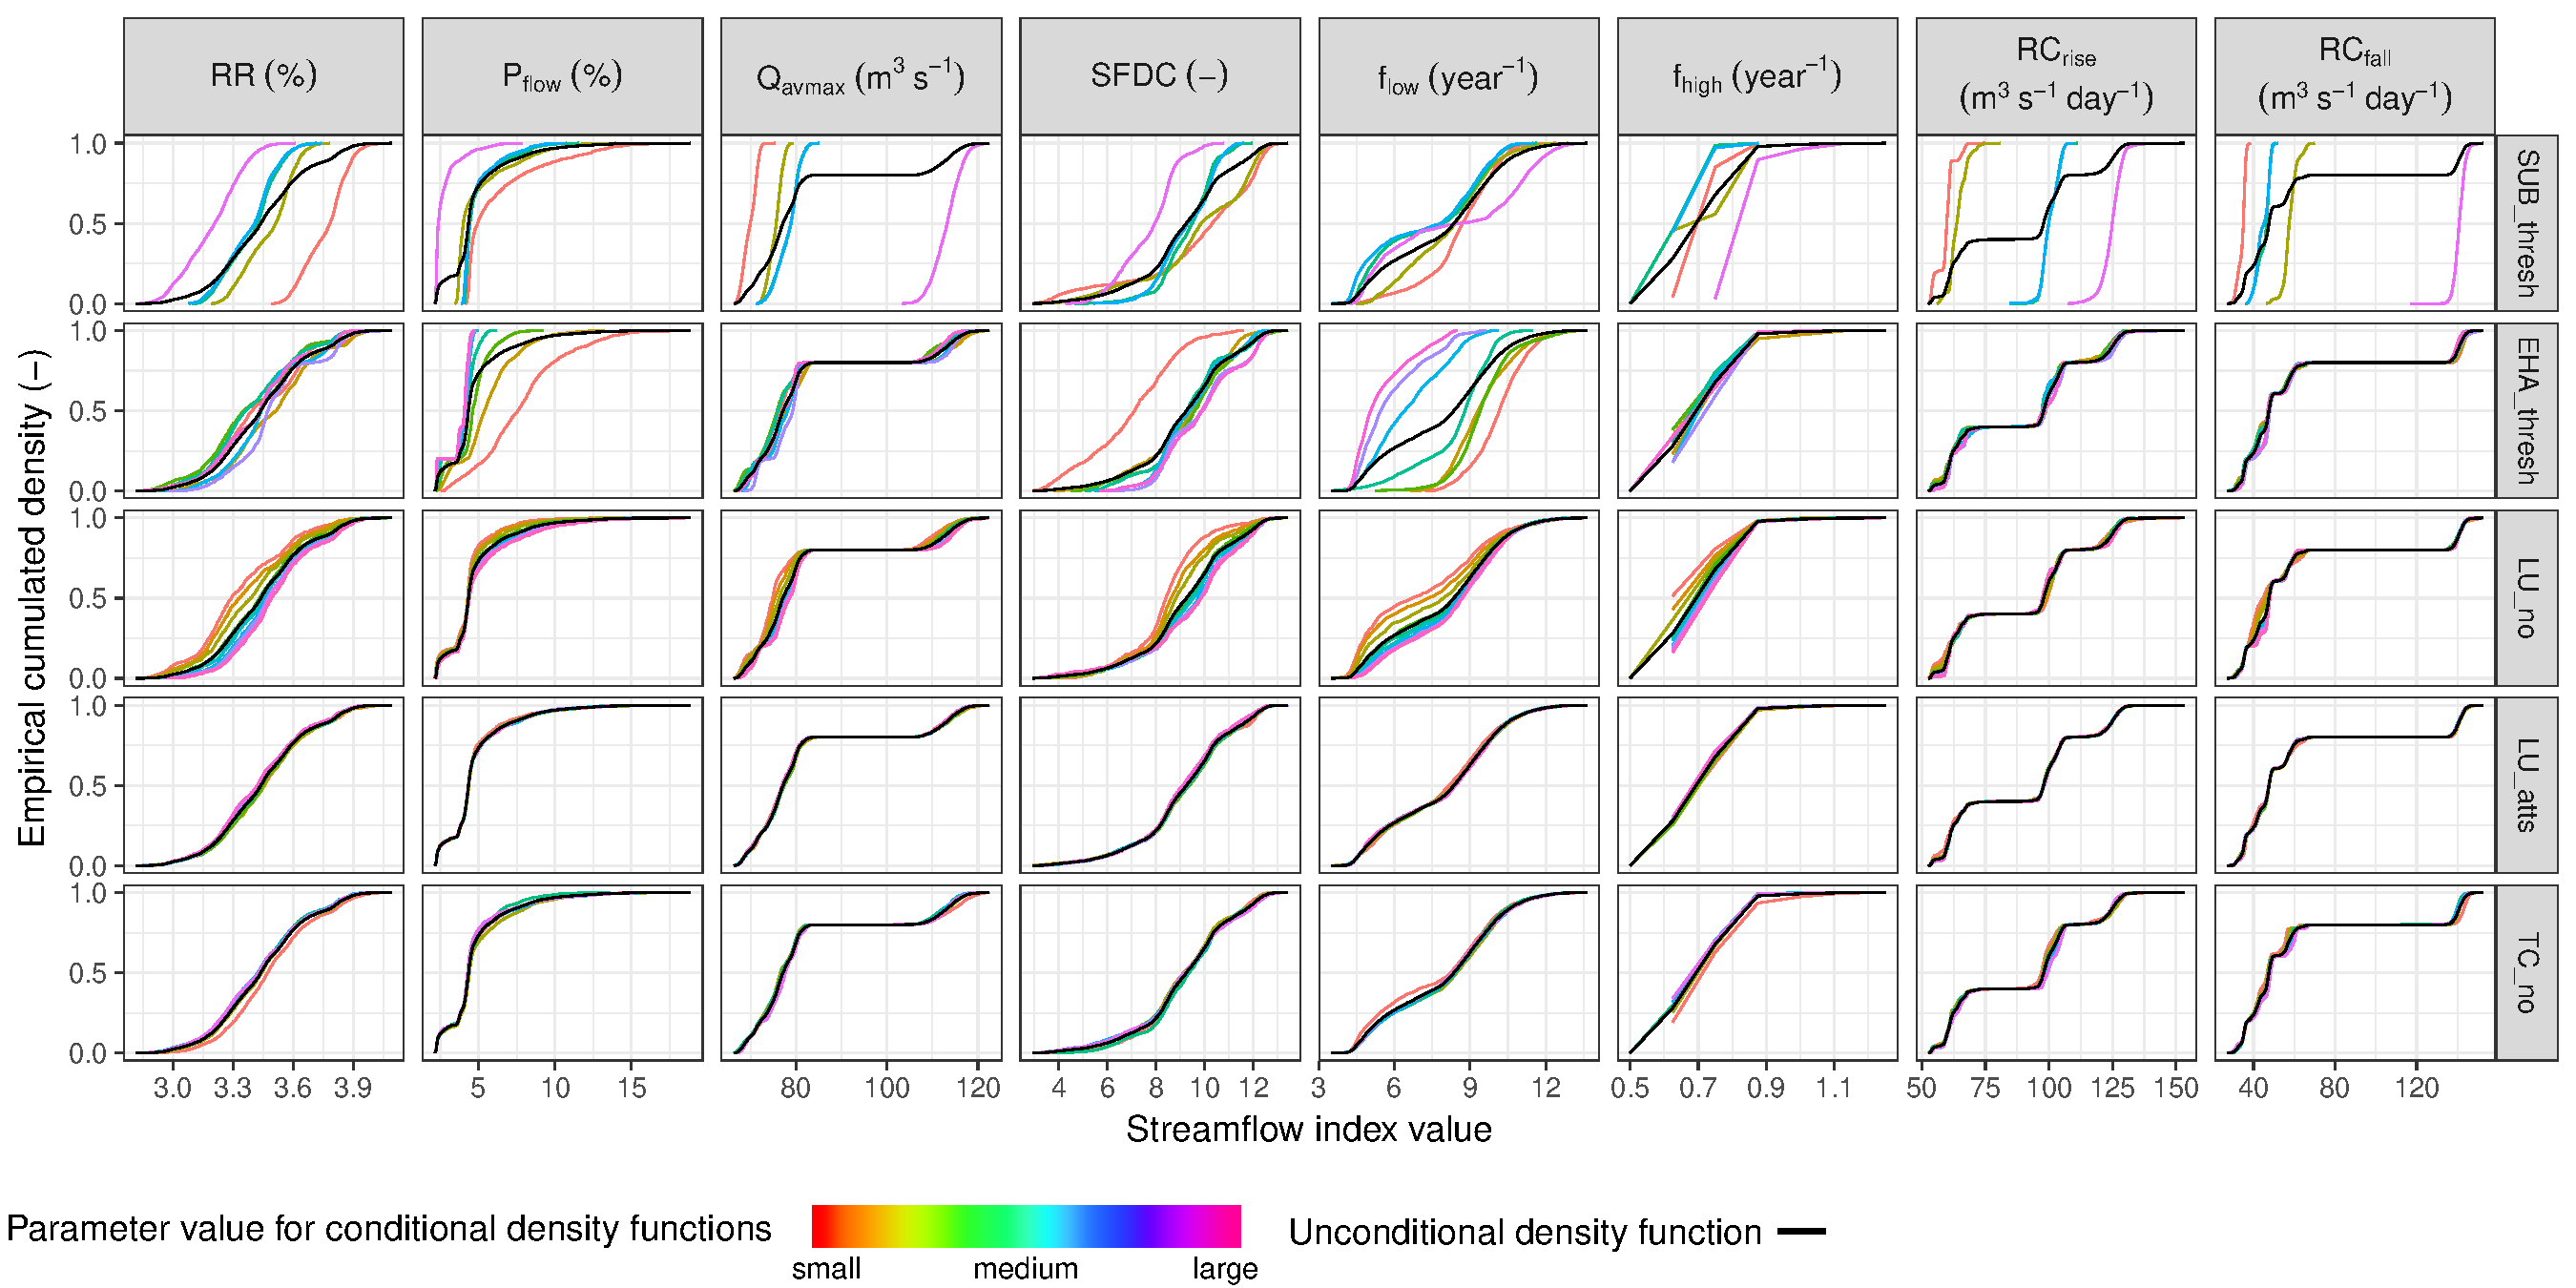
\includegraphics[width=\linewidth]{../analysis/sensitivity/sensitivity_PAWN_ecdf.pdf}
\caption{Unconditional (black lines) and conditional (rainbow coloured lines) empirical cumulative distribution functions for each streamflow index--discretisation parameter combination.}
\label{fig:PAWNecdf}
\end{figure*}

More information on parameter influences on the various streamflow indices can be obtained from Fig. \ref{fig:PAWNecdf}.
The more influential a parameter the more colourful a diagram, i.e., the larger the deviations of the conditional empirical cumulative distribution functions from the unconditional one.
Many of the diagrams show a clear relationship between parameter realisation and streamflow index value.
The larger the subbasins (i.e., the larger \verb!SUB_thresh! and the less the number of subbasins in the area) the smaller the generated amount of runoff ($RR$ gets smaller) and the smaller the probability of significant runoff ($P_{flow}$).
On the other hand, peak discharges ($Q_{avmax}$) increase and the catchment appears to produce more rapid runoff responses (higher values of $RC_{fall}$ and $RC_{rise}$).
Furthermore it can be seen that \verb!SUB_thresh! is responsible for the multi-modal distributions of $Q_{avmax}$, $f_{high}$, $RC_{fall}$, and $RC_{rise}$ as the conditional distribution functions show a less stepped shape than the unconditional functions.
The influence on $f_{low}$ appears to be less clear.
It can be seen, however, that larger values of \verb!SUB_thresh! result in a more pronounced bimodal distribution of that index.
Low flows are otherwise more dominated by the size of EHAs (\verb!EHA_thresh!).
The larger \verb!EHA_thresh! (i.e., the larger the EHAs and the lower their number) the less the probability for significant streamflow ($P_{flow}$) and the less the number of low flow events per year ($f_{low}$) while the flow regime becomes more variable (higher values of $SFDC$).
Higher numbers of LUs (\verb!LU_no!) result in more generated runoff ($RR$ increases) with a tendency to both higher frequencies of low flow and high flow events, and generate more variable streamflow regimes.




\section{Discussion}
\label{sec:discussion}

\subsection{lumpR: features, benefits, limitations}
It is still common practise for many researchers in the field of hydrological modelling to not automate their pre-processing steps and even if they do they write their own scripts which they do not distribute openly.
Furthermore, common limitations of existing software are that they are often model specific, and/or perform only certain steps of pre-processing, and/or are commercial or can only be used along with commercial software (e.g., ArcGIS or MATLAB).
On the other hand, the importance of FOSS GIS is increasing \citep[e.g.,][]{Steiniger2009, Branger2012}.
Our work tries to address these limitations and builds on the philosophy of FOSS.

With lumpR a supplemental package for the free and open-source programming language R has been developed.
It is a tool for the discretisation of landscapes for use along with hydrological computer models employing hierarchical spatial aggregation schemes with hillslopes as the fundamental terrain element.
The software has been so far tested under Windows as well Linux-based operating systems such as \mbox{openSUSE} and \mbox{Ubuntu}.
It is user-friendly in a way that it interacts with the GIS GRASS and thus allows graphical investigation and manual correction of outcomes.
Furthermore, it hides unnecessary detail from the user while at the same time ensuring a certain level of control over the discretisation process.
As R is a scripting language, model pre-processing in that way can easily be automated and reproduced.
Via the database tools the software allows to keep the output directories clearly arranged by putting all information into a database while supporting several database systems to do so.
On the other hand, depending on the user's needs, graphical outputs and files with intermediate results can be used for investigation or debugging.

Although in this study lumpR was tested together with the model WASA and the package provides a function to create the model's input files, it can be regarded as model independent.
First tests employing the simulation environment ECHSE \citep{Kneis2015} revealed the package to be easily adaptable for producing the input files needed by a specific model.
Furthermore, it is easily possible to manually export and arrange the values from the databases as needed.
Other candidate models are, in principal, all hydrological models with similarly complex spatial aggregation schemes as used by WASA that can make use of the information provided by lumpR, such as the WEPP model \citep{Flanagan1995}.\footnote{Readers considering lumpR for use with their model are encouraged to contact the corresponding author of this paper for support.}

The centrepiece of the package is the LUMP algorithm introduced by \citet{Francke2008} for the calculation of hillslope properties and the delineation of representative LUs together with the subdivision into TCs.
In contrast to simple GIS overlay techniques, as usually employed for the delineation of HRUs, it preserves information on the distribution of hillslope parameters and their relative topographic position.
In that way the task of landscape discretisation and parametrisation can be purposefully directed to landscape properties dominating hydrological response.
By the decision on certain parameter realisations it has been shown in the example application that descretisations of varying complexity can be easily produced.
A user can thus experiment and find out the optimal degree of complexity for a certain catchment and a specific objective, e.g., by systematically employing a multiple hypothesis framework.
Via its integration into lumpR the application of the algorithm could be further simplified and harmonised as the original LUMP consisted of a loose collection of less user-friendly scripts, partly also relying on non-free software such as MATLAB.
Furthermore, lumpR comes with a lot more additional functionalities than the mere LU and TC deviation.

Even so the package addresses a number of common limitations within existing software it is not free of constraints.
First of all its GRASS support is already deprecated as it builds, by the time of writing this paper, on GRASS version 6.4 whereas the first stable release of version 7 with a lot of improvements has been published in 2015.
However, due limited backwards compatibility the adaptation of lumpR demands a profound revision of the source code and is thus still planned as future enhancement.
This fact, however, comes with no further restriction except that a potential lumpR user will need to have the old GRASS 6.4 to be installed.
With regards to the applicability over large datasets, i.e., when applying the package to large areas in the order of >100,000 \unit{km^2} and/or when employing high-resolution DEMs, time consumption might pose a restriction.
Therefore, future enhancements also need to include improvements regarding computational efficiency.

A limitation more related to the algorithm is the restricted use of morphological parameters, currently limited to shape, horizontal and vertical extension, and hillslope width.
Future improvements should include the use of other factors relevant for hillslopes characterisation such as, for instance, contour curvature being related to the convergence or divergence of flowpaths and as such being of hydrological relevance \citep{Bogaart2006}.
Furthermore, the software is not able to automatically distinguish and account for artificial hydrological discontinuities such as ditches and field boundaries or other problematic formations such as large flat areas in a DEM as produced by lakes.
Such elements may negatively influence the delineation of hillslopes and LUs and should, if being of significant influence, be masked in GRASS before the analysis.
In addition, the pre- and post-processing steps within lumpR (i.e., functions \emph{lump\_grass\_prep()} and \emph{lump\_grass\_post()}) still partly suffer from imperfect or crude approaches.
This affects in particular the deviation of the river network, subbasin delineation, and the approximation of streamflow routing parameters (the latter tailored to the simplistic unit hydrograph approach of WASA).
In this respect future enhancements should also include a review on latest advancements of terrain analysis and parameterisation and the refinement of employed algorithms.


\subsection{On user decisions and sensitivity analysis}
As in science reproducibility and objectivity are primary criteria for any investigation it has to be noted that the LUMP algorithm, while providing some freedom of choices to the user, at the same time suffers from a certain degree of subjectivity.
This has been explicitly addressed via the sensitivity analysis within the example application and its results shall be discussed in the following.

The results from the 12,250 realisations of landscape discretisation show only little difference with respect to water storage dynamics of the Bangu\^e reservoir (Fig. \ref{fig:resvol}).
The small variation of the runoff coefficient (cf.\ Fig. \ref{fig:hydIndices}) further supports the conclusion that decisions on landscape discretisation parametrisation only have a minor impact on simulated runoff volume.
On the other hand, the influence on other indices describing runoff concentrations and dynamics, and the frequency of flood or drought events is much more obvious.

The hydrological regime of the study area is primarily influenced by precipitation which is characterised by a high temporal concentration and a large temporal and spatial variability.
A comparison with the data reported in \citet{Medeiros2014b} further supports that uncertainties regarding the precipitation input to the model have a much larger impact on simulation results than user decisions on LUMP parameters.
In their study \citet{Medeiros2014b} used a set of raw station data in contrast to the preprocessed and gridded dataset by \citet{Xavier2016} used for our experiments and their runoff values have been assessed by taking the Bengu\^e reservoir inflows computed from water balance calculations.
Their reported runoff coefficients are mostly lower than ours, even when precipitation is higher, and shows less inter-annual variation (see Fig. \ref{fig:prec_rc_compare} in Appendix).
The precipitation forcing for the experiments was implicitly influenced by variable subbasin sizes and numbers as the WASA model derived rainfall input at the subbasin level.
The variability in precipitation input among the experiments, however, appears to be negligible as it is generally less than 6 \unit{mm} for daily values and less than 10 \unit{mm} for yearly sums (see Fig. \ref{fig:prec_diff} in Appendix).

Regarding the method of sensitivity analysis it can be concluded that the choice for a density-based approach was reasonable as most of the analysed streamflow indices exhibit multi-modal or skewed value distributions.
Furthermore, the interpretation of the PAWN index proofed to be straightforward.
On the other hand, also the whole parameter range has been sampled, the definition of reasonable ranges was based on subjective decisions and data availability.
Another drawback on the analysis approach is that only first order effects of parameter sensitivities have been quantified while interactions among parameters have been neglected.
It might thus be that insignificant parameters (i.e., the parameter \verb!LU_atts!) have significant higher order effects due to parameter correlations. 

Overall, the example study and sensitivity analysis was strongly case study specific and conclusions are thus limited to regions with similar hydro-climatic conditions, i.e., semi-arid areas without substantial groundwater influences mainly characterised by spatially and temporally heterogeneous precipitation patterns.


\TP[inline]{Does the Discussion section already contain too much conclusions?}

%- SA method:
%- many of the analysed indices exhibit multi-modal or skewed distributions -> density-based approach
%- the whole parameter range was sampled
%- uncertainty in the definition of a feasible parameter range 
%
%- findings strongly case-study specific, more case studies under different hydro-climatic conditions needed for general conclusions




\conclusions  %% \conclusions[modified heading if necessary]
\label{sec:conclusions}
TODO




\section{Code availability}
\label{sec:code_availability}
TODO




\section{Data availability}
Meteorological data are available from \url{http://careyking.com/data-downloads/}.
DEM raw data can be obtained via \url{http://srtm.csi.cgiar.org/SELECTION/inputCoord.asp} by selecting tile 28/14 (horizontal/vertical).
Reservoir data and the geology map have been processed within the SESAM project and are not publicly available.
For more information and contact details see \url{http://www.uni-potsdam.de/sesam}.
Land cover and soil raster maps are not publicly available.





\newpage
\appendix
\section{Precipitation uncertainty and comparisons with other studies}    %% Appendix A
\TP[inline]{Figures herein are still preliminary and need adjustments (legend, larger font size etc.).}

\appendixfigures  %% needs to be added in front of appendix figures in one-column style (\documentclass[acp, manuscript]{copernicus})

\begin{figure*}[h]
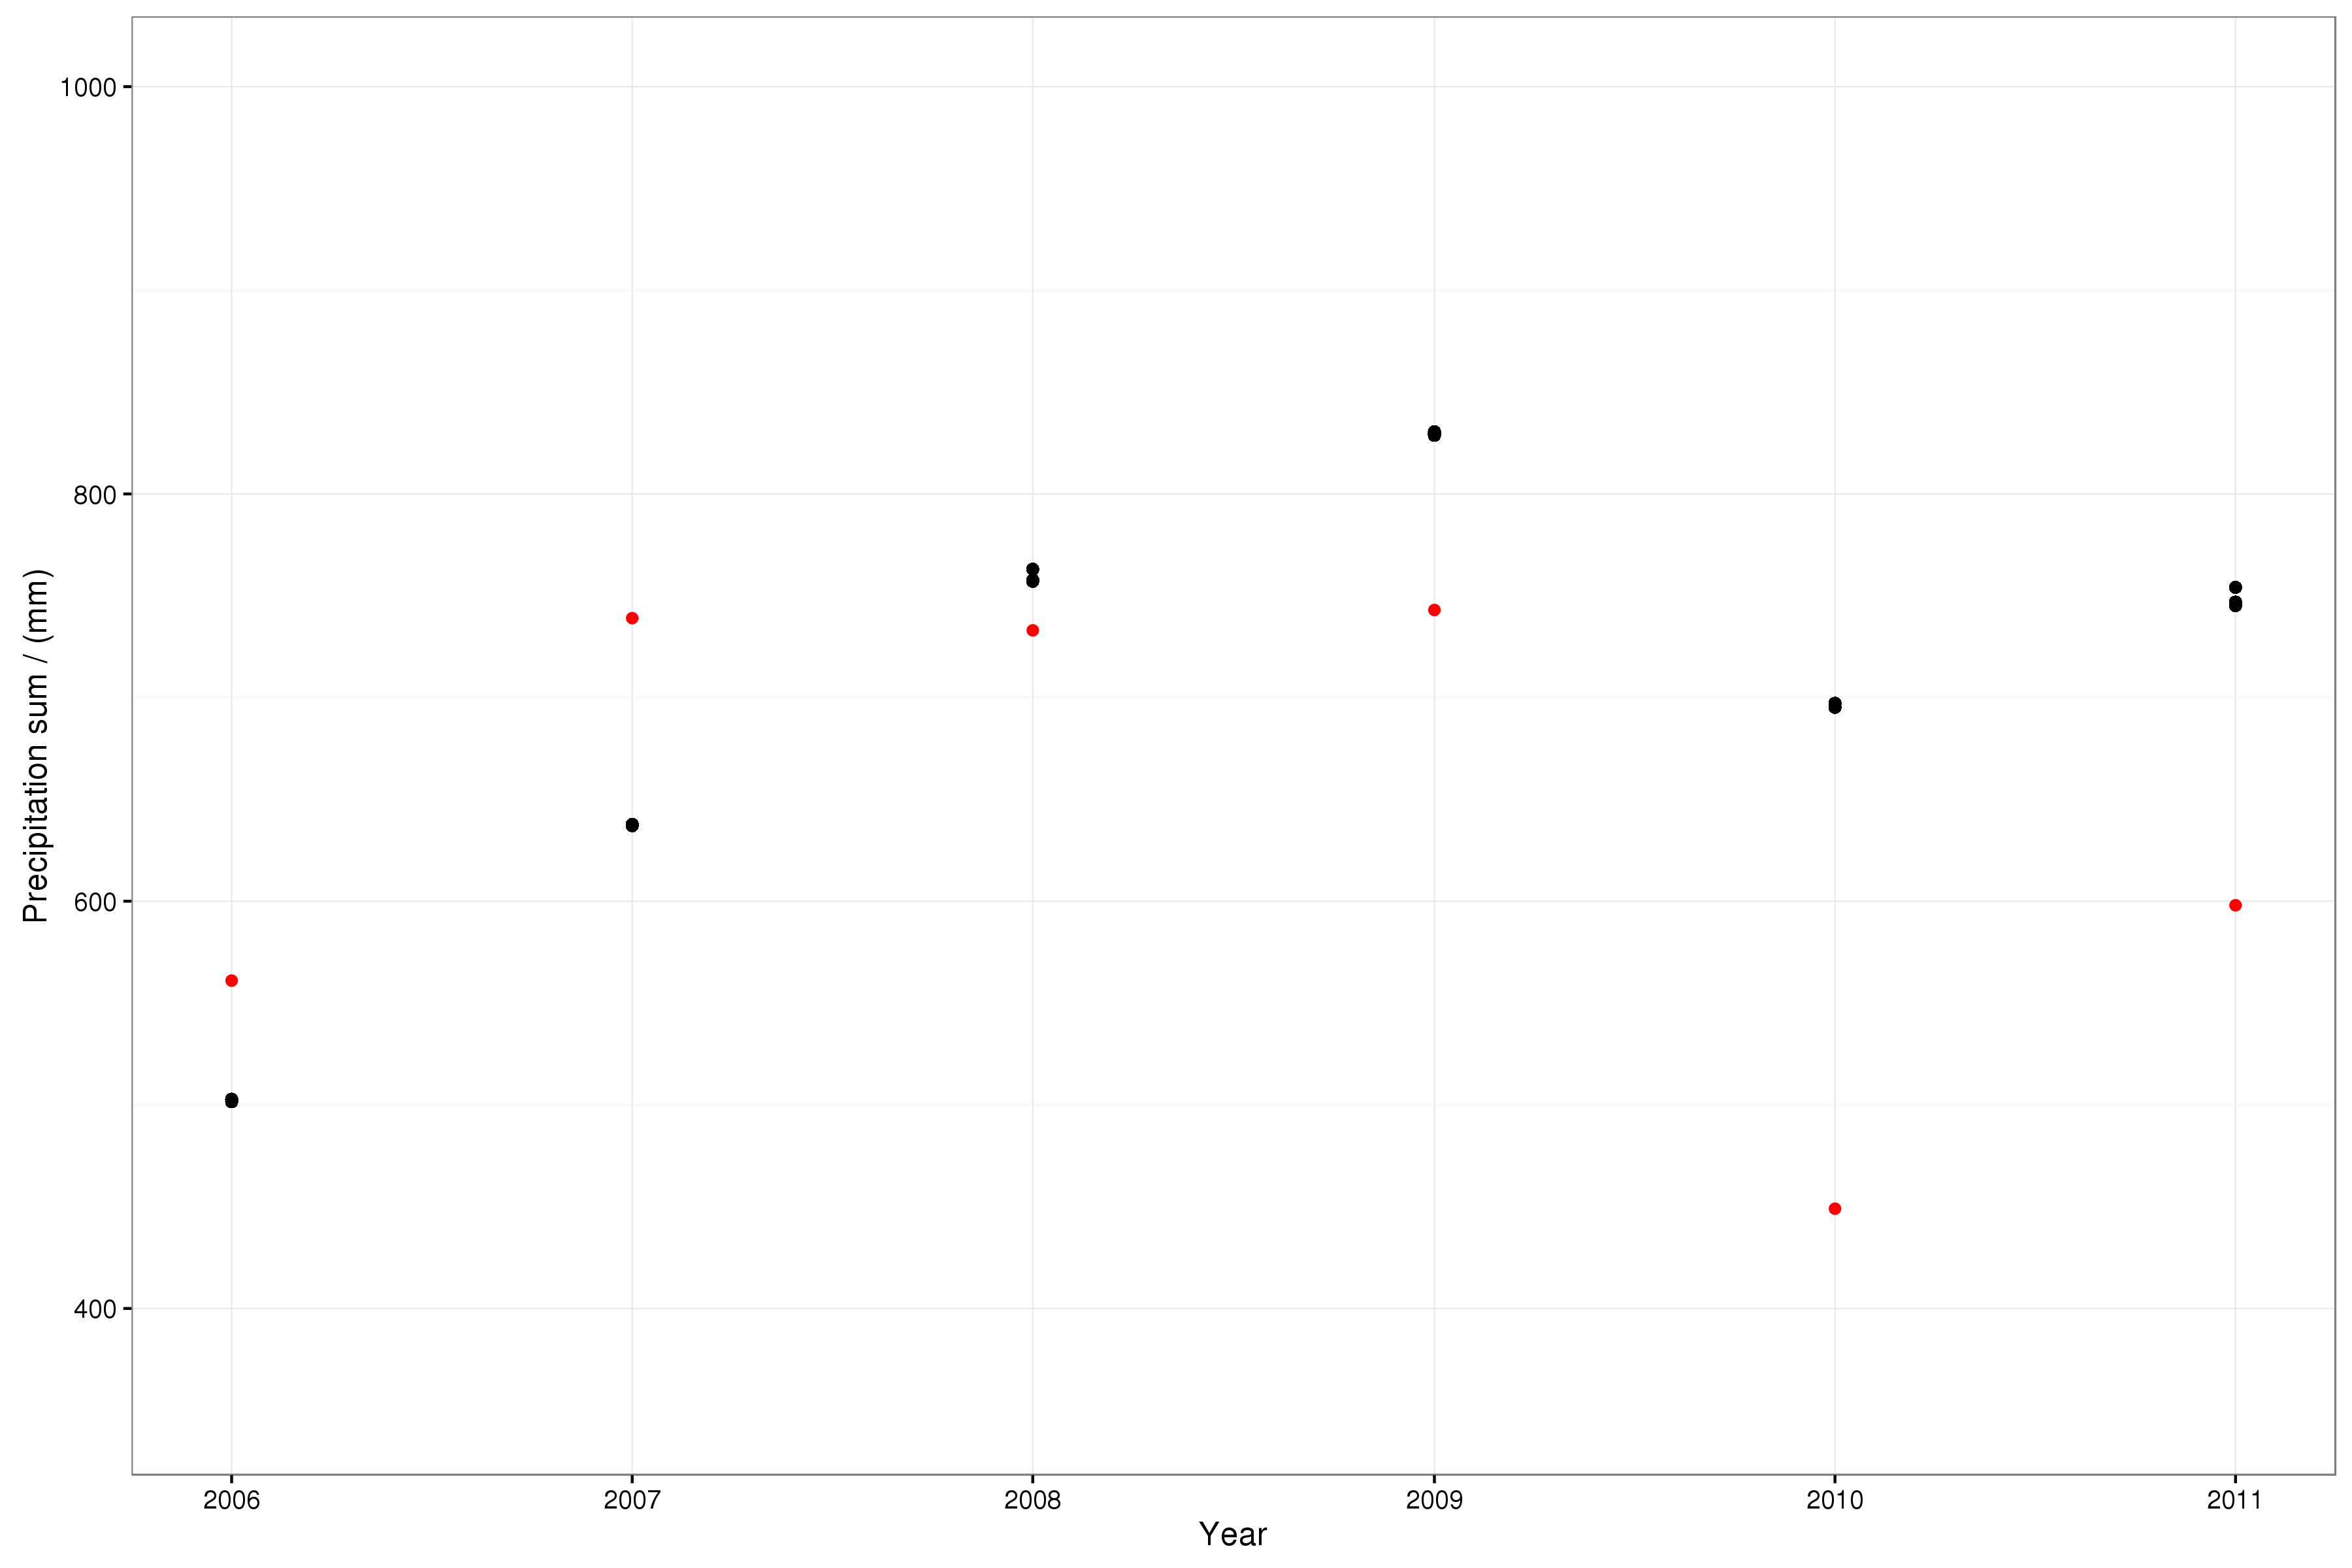
\includegraphics[width=.45\linewidth]{../analysis/comparison_results/Bengue_prec_compare.png}
\hfill
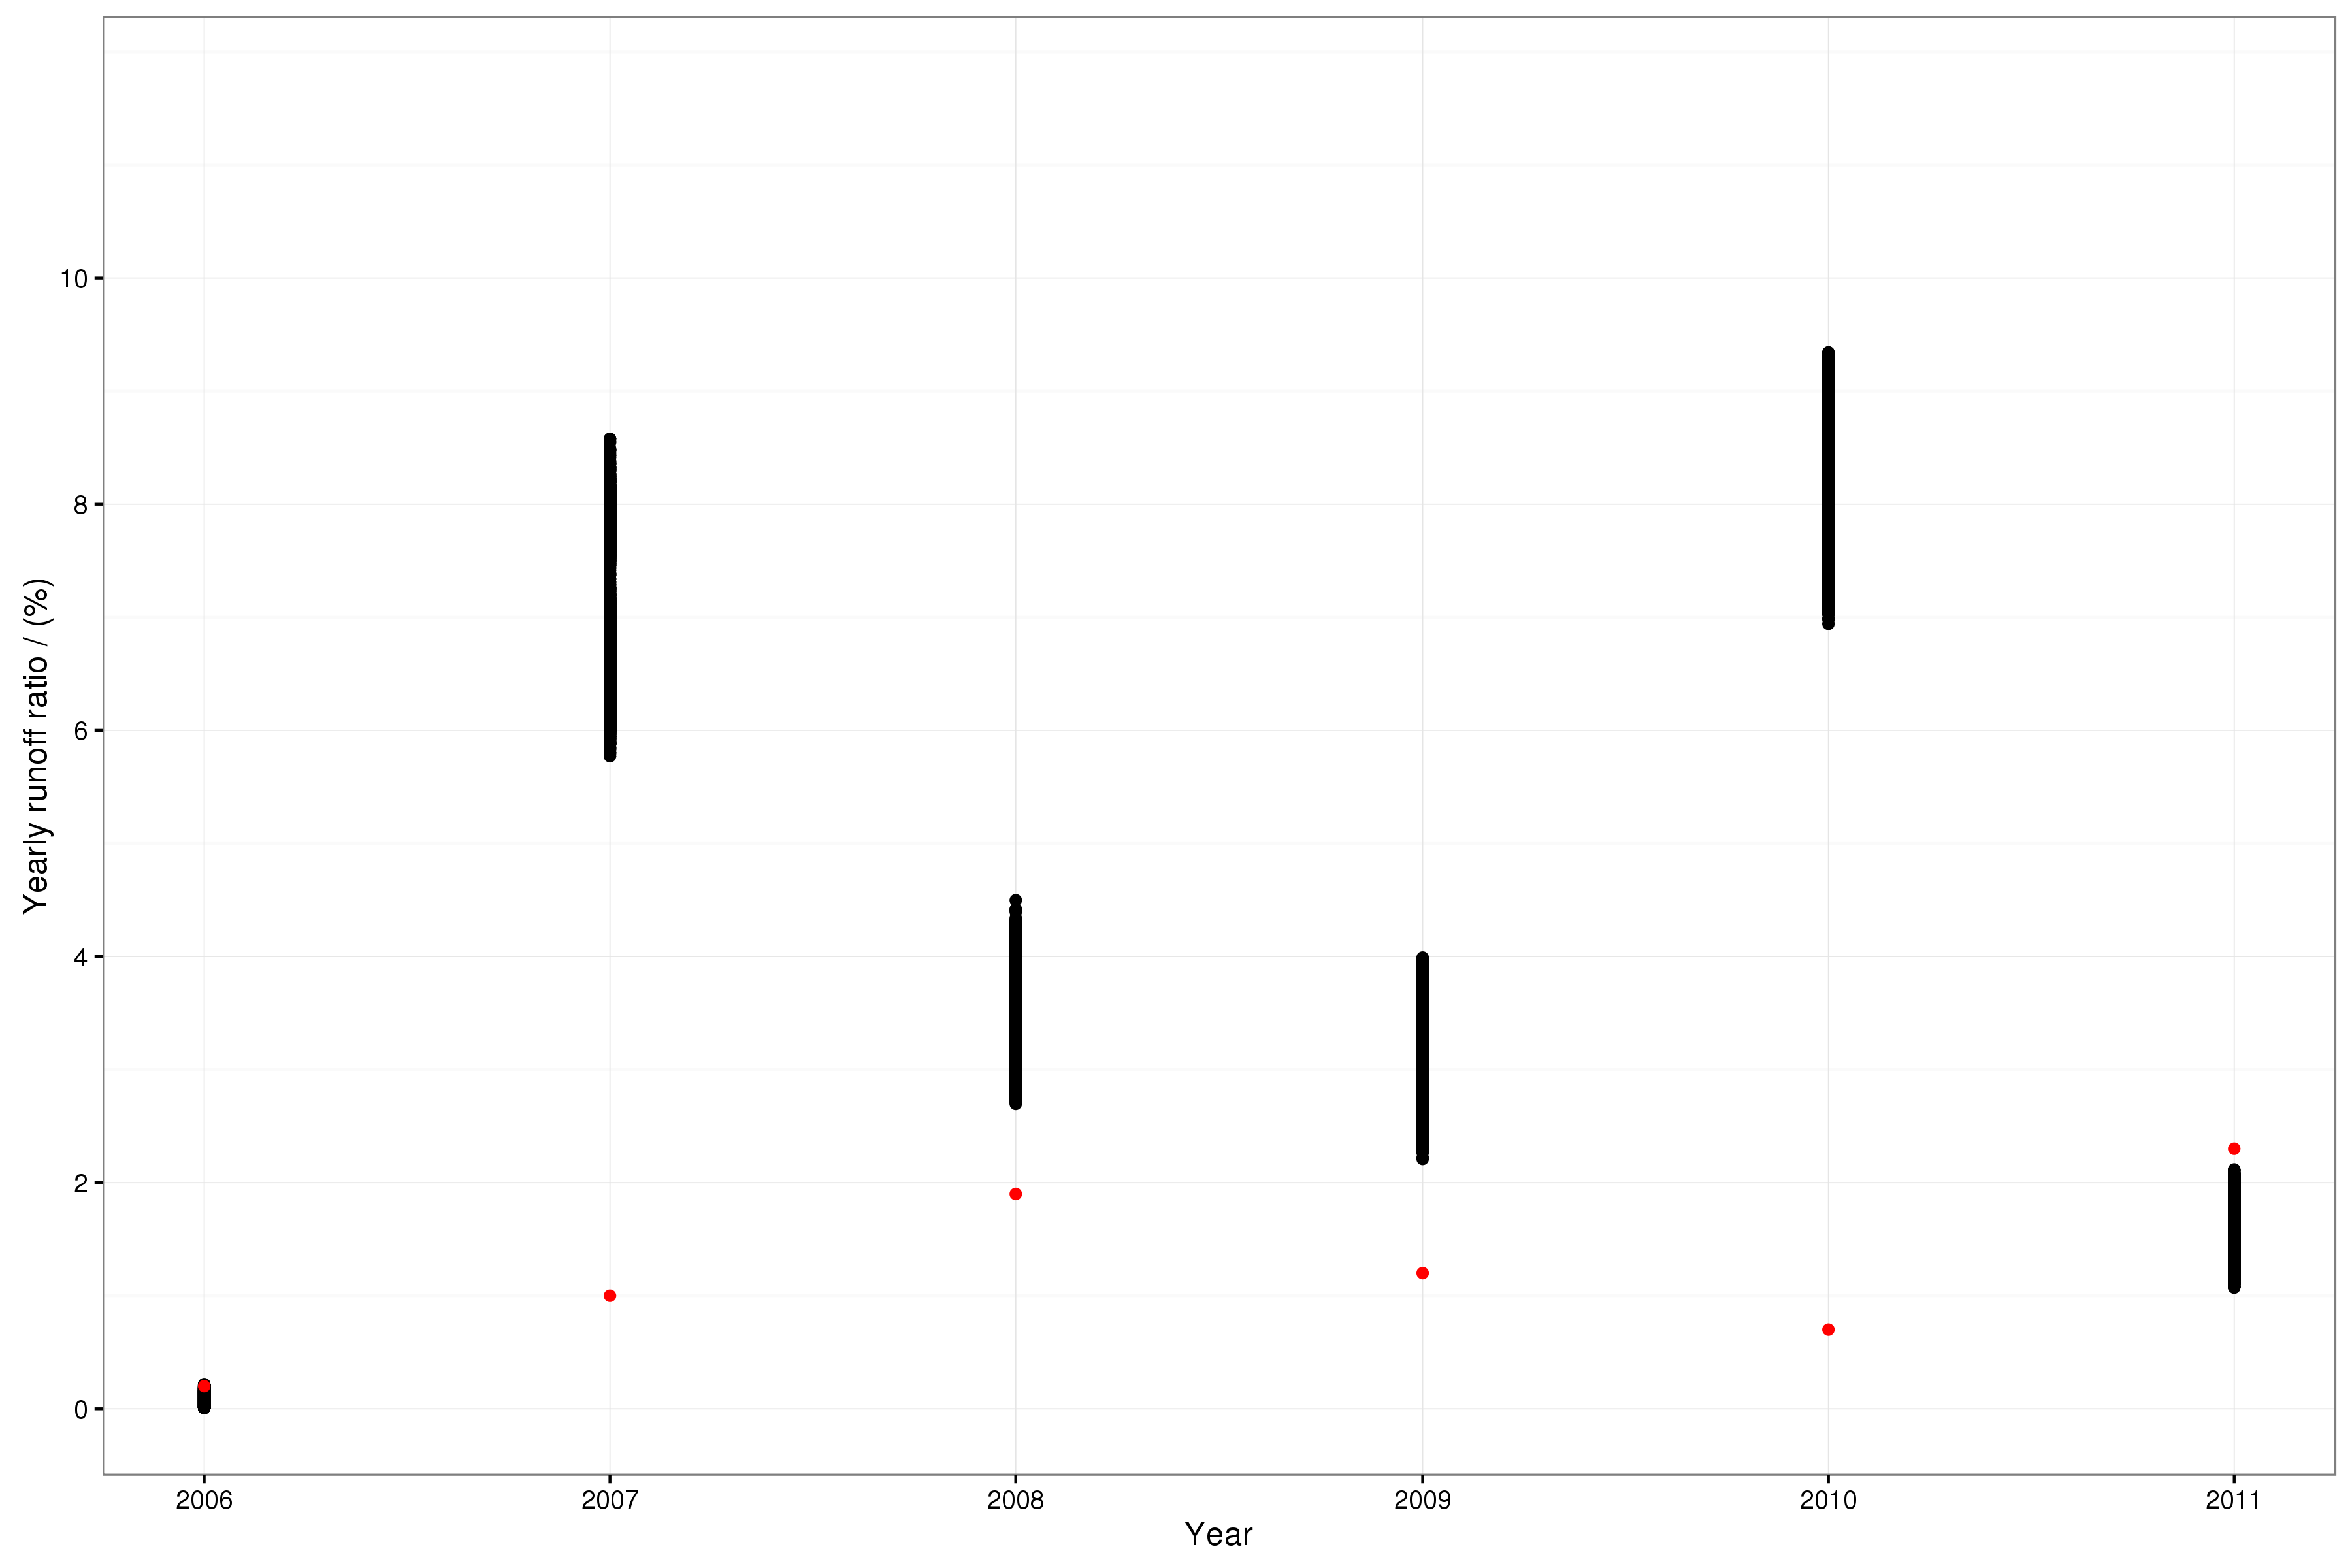
\includegraphics[width=.45\linewidth]{../analysis/comparison_results/Bengue_rc_compare.png}
\caption{Comparison of precipitation forcing (left) and simulated yearly runoff coefficients (right) with values reported by \citet{Medeiros2014b} (red dots).}
\label{fig:prec_rc_compare}
\end{figure*}

\begin{figure*}[h]
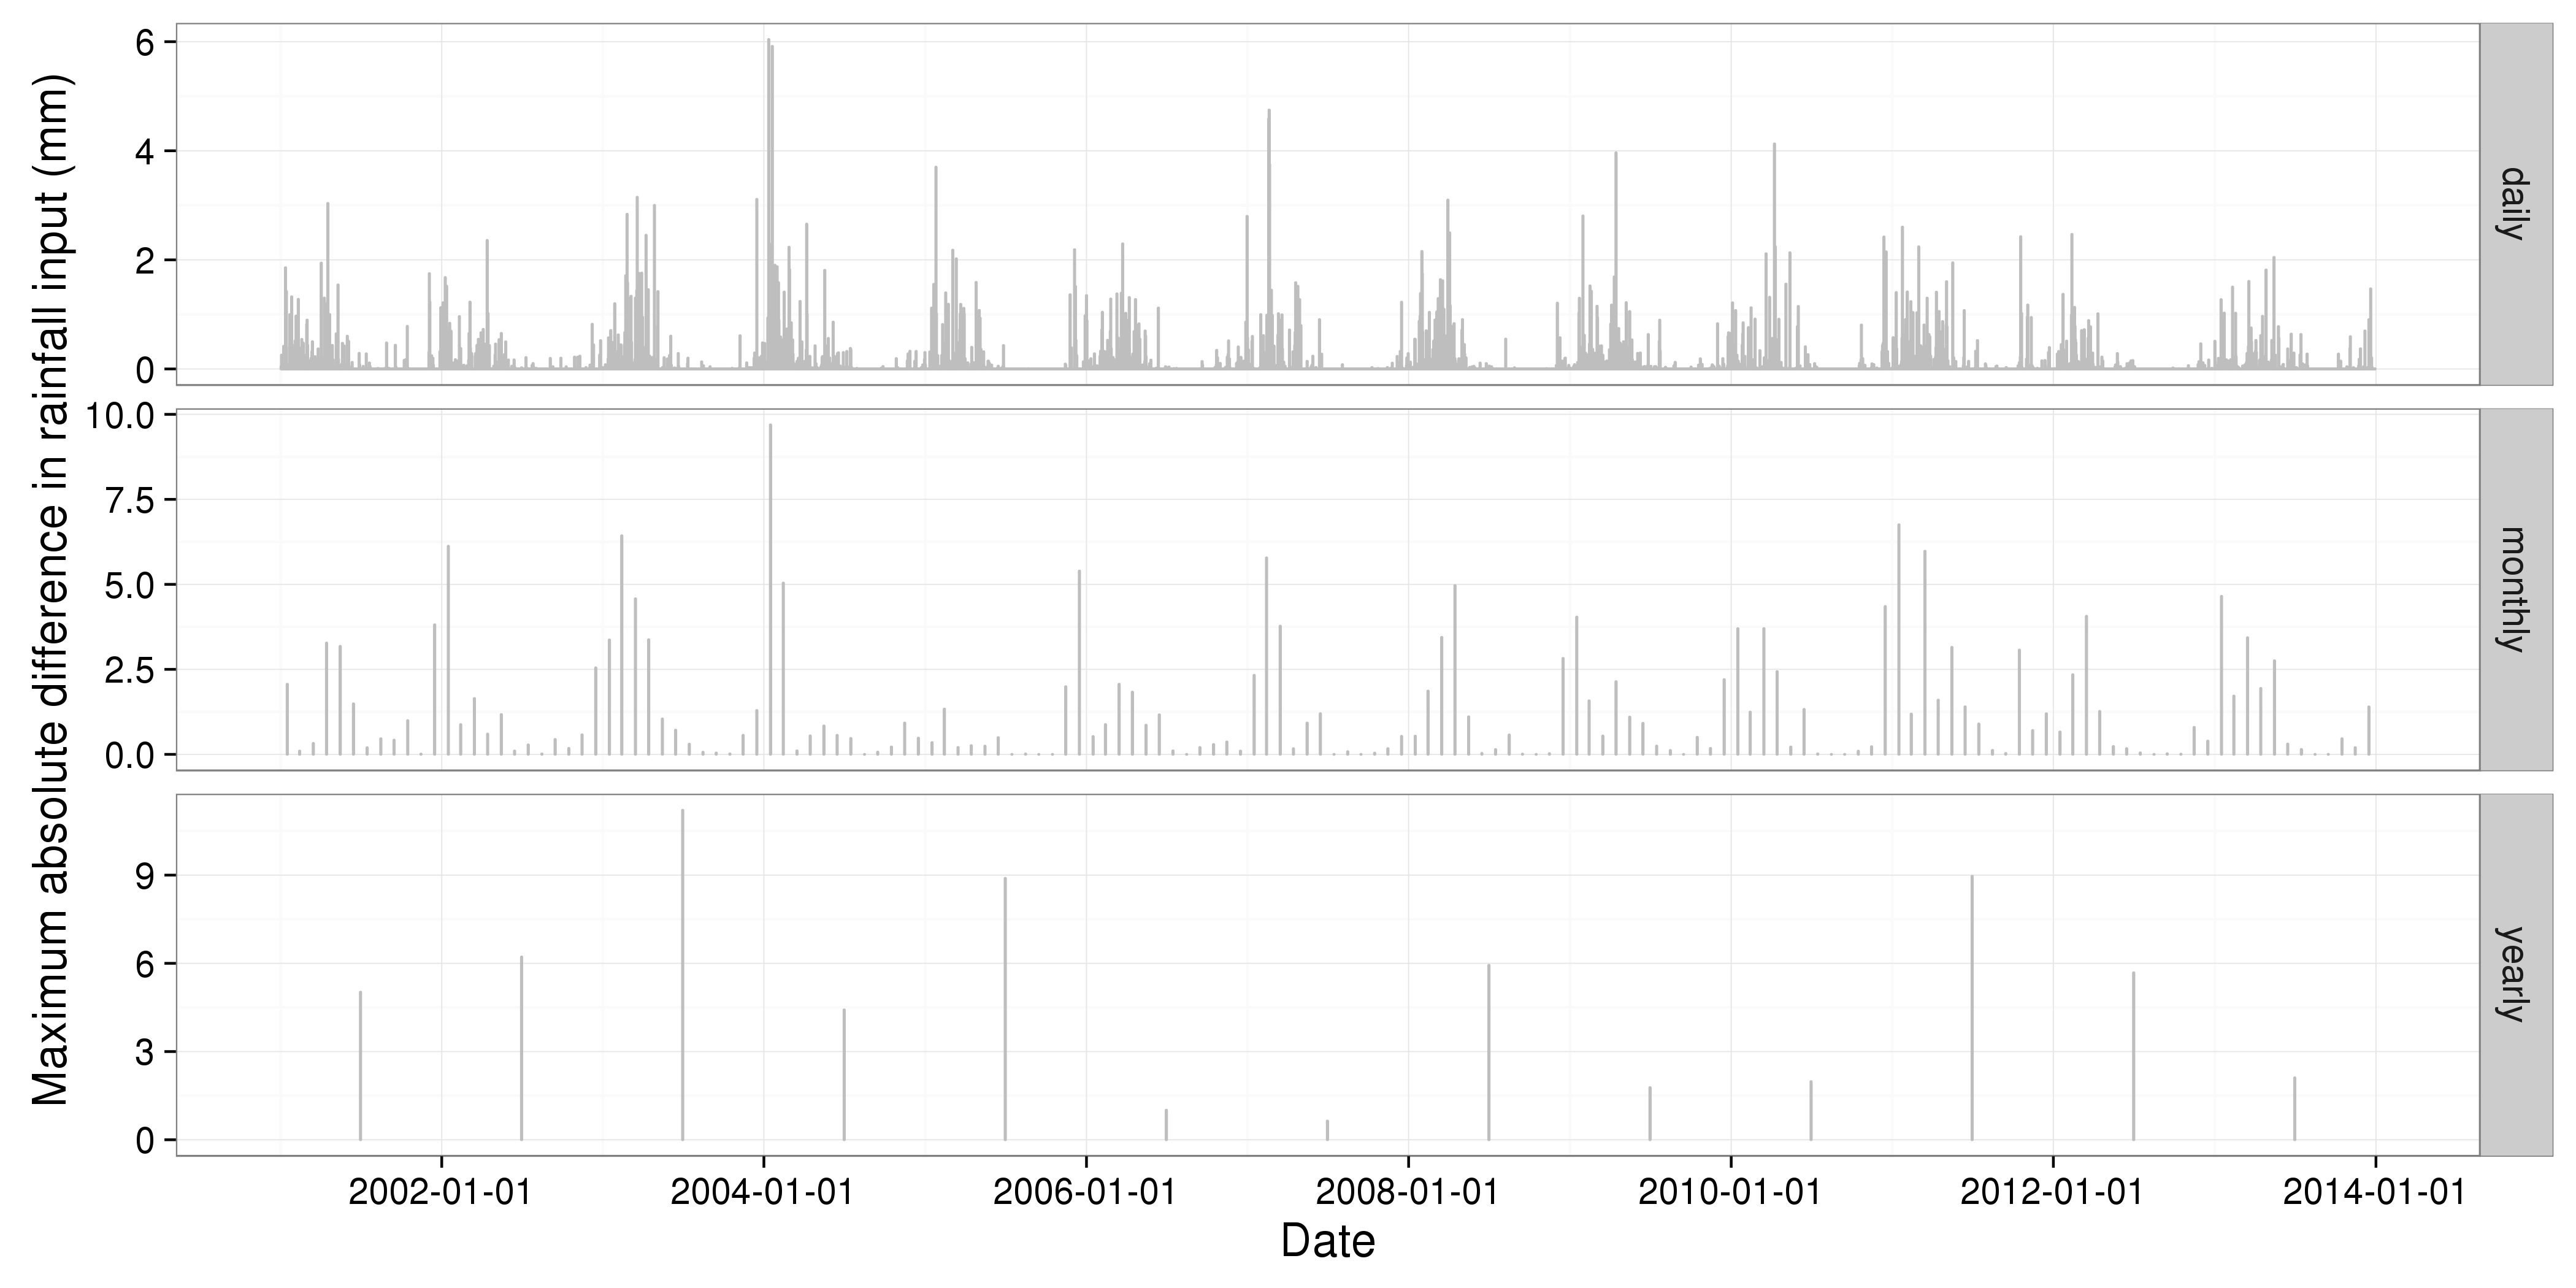
\includegraphics[width=.95\linewidth]{../analysis/comparison_results/rainfall_maxabsdiff_experiments_overview.png}
\caption{Maximum of absolute differences in rainfall between the 12,250 experiments for every time step.}
\label{fig:prec_diff}
\end{figure*}


\appendixtables   %% needs to be added in front of appendix tables in one-column style (\documentclass[acp, manuscript]{copernicus})




\authorcontribution{TODO}

%\competinginterests{TEXT}
%
%\disclaimer{TEXT}

\begin{acknowledgements}
Authors thank Fernanda Scholz (former M.Sc. student at the Leibniz University of Hannover) for the preparation of soil data.
M. Sc. student Lisa Bergh\"auser from the University of Potsdam is acknowledged for testing lumpR within her Thesis and giving valuable feedback and bug reports.
Tobias Pilz acknowledges funding by the Helmholtz graduate school GeoSim.
\TP{Any more acknowledgements from your side?}
\end{acknowledgements}



%% REFERENCES

\bibliographystyle{copernicus}

\bibliography{references}


%% Since the Copernicus LaTeX package includes the BibTeX style file copernicus.bst,
%% authors experienced with BibTeX only have to include the following two lines:
%%
%% \bibliographystyle{copernicus}
%% \bibliography{example.bib}
%%
%% URLs and DOIs can be entered in your BibTeX file as:
%%
%% URL = {http://www.xyz.org/~jones/idx_g.htm}
%% DOI = {10.5194/xyz}


%% LITERATURE CITATIONS
%%
%% command                        & example result
%% \citet{jones90}|               & Jones et al. (1990)
%% \citep{jones90}|               & (Jones et al., 1990)
%% \citep{jones90,jones93}|       & (Jones et al., 1990, 1993)
%% \citep[p.~32]{jones90}|        & (Jones et al., 1990, p.~32)
%% \citep[e.g.,][]{jones90}|      & (e.g., Jones et al., 1990)
%% \citep[e.g.,][p.~32]{jones90}| & (e.g., Jones et al., 1990, p.~32)
%% \citeauthor{jones90}|          & Jones et al.
%% \citeyear{jones90}|            & 1990



%% FIGURES

%% We suggest to put the figures in the correct order and placement within the text. This aids readability.
%% When figures and tables are placed at the end of the MS (article in one-column style), please add \clearpage
%% between bibliography and first table and/or figure as well as between each table and/or figure.


%% ONE-COLUMN FIGURES

%%f
%\begin{figure}[t]
%\includegraphics[width=8.3cm]{FILE NAME}
%\caption{TEXT}
%\end{figure}
%
%%% TWO-COLUMN FIGURES
%
%%f
%\begin{figure*}[t]
%\includegraphics[width=12cm]{FILE NAME}
%\caption{TEXT}
%\end{figure*}
%
%
%%% TABLES
%%%
%%% The different columns must be seperated with a & command and should
%%% end with \\ to identify the column brake.
%
%%% ONE-COLUMN TABLE
%
%%t
%\begin{table}[t]
%\caption{TEXT}
%\begin{tabular}{column = lcr}
%\tophline
%
%\middlehline
%
%\bottomhline
%\end{tabular}
%\belowtable{} % Table Footnotes
%\end{table}
%
%%% TWO-COLUMN TABLE
%
%%t
%\begin{table*}[t]
%\caption{TEXT}
%\begin{tabular}{column = lcr}
%\tophline
%
%\middlehline
%
%\bottomhline
%\end{tabular}
%\belowtable{} % Table Footnotes
%\end{table*}
%
%
%%% MATHEMATICAL EXPRESSIONS
%
%%% All papers typeset by Copernicus Publications follow the math typesetting regulations
%%% given by the IUPAC Green Book (IUPAC: Quantities, Units and Symbols in Physical Chemistry,
%%% 2nd Edn., Blackwell Science, available at: http://old.iupac.org/publications/books/gbook/green_book_2ed.pdf, 1993).
%%%
%%% Physical quantities/variables are typeset in italic font (t for time, T for Temperature)
%%% Indices which are not defined are typeset in italic font (x, y, z, a, b, c)
%%% Items/objects which are defined are typeset in roman font (Car A, Car B)
%%% Descriptions/specifications which are defined by itself are typeset in roman font (abs, rel, ref, tot, net, ice)
%%% Abbreviations from 2 letters are typeset in roman font (RH, LAI)
%%% Vectors are identified in bold italic font using \vec{x}
%%% Matrices are identified in bold roman font
%%% Multiplication signs are typeset using the LaTeX commands \times (for vector products, grids, and exponential notations) or \cdot
%%% The character * should not be applied as mutliplication sign
%
%
%%% EQUATIONS
%
%%% Single-row equation
%
%\begin{equation}
%
%\end{equation}
%
%%% Multiline equation
%
%\begin{align}
%& 3 + 5 = 8\\
%& 3 + 5 = 8\\
%& 3 + 5 = 8
%\end{align}
%
%
%%% MATRICES
%
%\begin{matrix}
%x & y & z\\
%x & y & z\\
%x & y & z\\
%\end{matrix}
%
%
%%% ALGORITHM
%
%\begin{algorithm}
%\caption{�}
%\label{a1}
%\begin{algorithmic}
%�
%\end{algorithmic}
%\end{algorithm}
%
%
%%% CHEMICAL FORMULAS AND REACTIONS
%
%%% For formulas embedded in the text, please use \chem{}
%
%%% The reaction environment creates labels including the letter R, i.e. (R1), (R2), etc.
%
%\begin{reaction}
%%% \rightarrow should be used for normal (one-way) chemical reactions
%%% \rightleftharpoons should be used for equilibria
%%% \leftrightarrow should be used for resonance structures
%\end{reaction}
%
%
%%% PHYSICAL UNITS
%%%
%%% Please use \unit{} and apply the exponential notation


\end{document}
